%% Road to VPhO 2023 Template

\documentclass[12pt]{article}
% \usepackage[english]{babel}
\usepackage[utf8]{vietnam}
\usepackage[T5]{fontenc}
\usepackage[top=2cm, bottom=2cm, left=2cm,right=2cm]{geometry}
%% Margin %%

%%%%%%%%%% Figure %%%%%%%%%%%%%
\usepackage[pdftex]{graphicx}
\usepackage{subcaption}
\usepackage{wrapfig}

\usepackage[dvipsnames]{xcolor}
\usepackage[pdftex]{graphicx}
\usepackage{wrapfig}
\usepackage{tcolorbox}
\usepackage{mathtools}
\usepackage{amsmath}
\usepackage{amssymb}
\usepackage{eqnarray}
\usepackage{siunitx}
\usepackage{array, lipsum, bibentry,fancyhdr}
\usepackage{hyperref}
\usepackage{natbib}
\setlength{\parindent}{0pt}
\usepackage{enumitem}
\usepackage[noframe]{showframe}
\usepackage{framed}
\usepackage{titling}
\usepackage{float}
\usepackage{multicol}
\usepackage{url}
\usepackage{authblk}
\usepackage{sectsty}
\usepackage{eqparbox}

%%%%%%%%%% Pictures drawing %%%%%%%%%%%%%

\usepackage{pgfplots} %%%%%% Regression %%%%
\pgfplotsset{compat = newest}
\usepackage{pgfplotstable}
\usepackage{tikz}
\usepackage{tikz-3dplot} %%%%%% Draw %%%%%%
\usepackage{tikz,tkz-euclide}
\usetikzlibrary{arrows,calc,patterns}
\usetikzlibrary{quotes,angles}
\usetikzlibrary{shapes.geometric}
\usepackage{circuitikz} %%%%% Circuit %%%%
\usetikzlibrary{decorations.pathmorphing,patterns}

\setlength{\unitlength}{1cm}

%%%%%%%%%% Hyperlink %%%%%%%%%%%%%

\hypersetup{
	colorlinks=true,
	linkcolor=black,
	filecolor=mangeta,      
	urlcolor=blue,
	pdftitle={Overleaf Example},
	pdfpagemode=FullScreen,
}

%%%%%%%%%% Header & Footer %%%%%%%%%%%%%

\setlength{\headheight}{10mm}
\RequirePackage{fancyhdr}  % Needed to define custom headers/footers
\RequirePackage{lastpage}  % Number of pages in the document
\pagestyle{fancy}          % Enables the custom headers/footers
% Headers
\lhead{
\includegraphics[width=.8in]{xPhO.png}}%
\chead{}%
\rhead{\small\sffamily\bfseries{Lời giải hướng tới VPhO 44} --- \thepage/\pageref{LastPage}}
% Footers
\lfoot{}%
\cfoot{}%
\rfoot{}%
\renewcommand{\headrulewidth}{1pt}% % header rule
\renewcommand{\footrulewidth}{1pt}% % footer rule

% \pagestyle{fancy}
% 	\fancyhead[L]{\empty}
% 	\fancyhead[R]{\empty}
% 	\fancyhead[C]{\empty}
% 	\fancyfoot[C]{\empty}
% 	\fancyfoot[L]{\empty}
% 	\renewcommand{\headrulewidth}{0pt}
% 	\fancyfoot[C]{\normalcolor{\thepage/\pageref{LastPage}}}
% 	\setcounter{page}{1}

%%%%%%%%%% Color setup %%%%%%%%%%%%%

\RequirePackage{xcolor}
\definecolor{wsdred}{HTML}{8E1728}
\definecolor{wsdgrey}{HTML}{75787B}
\renewcommand{\normalcolor}{\color{wsdred}}
\colorlet{ColorOr}{white}

\begin{document}

%% Title %%
{\fontsize{50}{24}\fontfamily{phv}\fontseries{b}
\LARGE \normalcolor{ \textbf{Đề hướng tới VPhO 44} } }

\textcolor{blue}{\textbf{\textit{Câu lạc bộ vật lý xPhO}}}

%%%%
\vspace{5mm}

{\normalcolor\textbf{CÂU 1.}}\vspace{1.5mm}

\setcounter{equation}{0}
Một quả lựu đạn đang đứng yên ở độ cao $H$ so với mặt đất thì phát nổ và bắn ra các mảnh đạn giống nhau với cùng tốc độ $v_0$, phân bố các mảnh đạn khi văng ra là đẳng hướng. Gia tốc trọng trường là $\Vec{g}$.
\begin{enumerate}[label=\textbf{\alph*,}]\itemsep0em
    \item Xác định phương trình mặt cong ba chiều biểu diễn ranh giới giữa \textit{vùng an toàn} và \textit{vùng nguy hiểm}, tức là trong vùng an toàn thì mảnh đạn sẽ không thể bay tới, ngược lại với vùng nguy hiểm. Vẽ phác dạng đồ thị của đường ranh giới, ghi chú thích và các điểm đặc biệt.
    \item Sau khi các mảnh đạn rơi hết xuống đất, xác định bán kính $R$ của vùng đạn đã rơi trên mặt đất.
    \item Giả sử rằng lựu đạn chứa $M$ khối lượng đạn nổ trong một góc nón nhỏ hướng lên trên với góc mở $2\alpha_0 \ll 1$, bom nổ trên mặt đất ($H = 0$). Chứng minh rằng phân bố khối lượng mặt $\rho(r)$ (khai triển tới thành phần bậc hai $r^2$) của đạn trên mặt đất khi tất cả mảnh đạn đã rơi xuống đất có dạng như sau
    $$\rho(r) \approx \rho_0 (1 + \beta r^2),$$

    hãy biểu diễn $\rho_0$ và $\beta$ theo các thông số đã biết.
\end{enumerate}

\textit{Có thể sử dụng xấp xỉ sau:} $\displaystyle \sin \alpha \approx \alpha \left(1 - \frac{1}{6} \alpha^2 \right)$.

\begin{flushright}
    (Biên soạn bởi Zinc)
\end{flushright}
\setcounter{equation}{0}
% \begin{center}
%     \normalcolor{\textbf{Bài giải}}
% \end{center}
% \textbf{a,} Ta đặt $r = \sqrt{x^2 + y^2}$ là toạ độ khoảng cách trong mặt phẳng $Oxy$. Từ phương trình ném xiên, tuân theo định luật Newton II, ta có phương trình chuyển động của mảnh đạn:
\begin{align}
    z &= -\frac{1}{2} g t^2 + v_0 \sin \theta t + H, \label{1}\\
    r&= v_0 \cos \theta t. \label{2}
\end{align}

Thay (\ref{1}) vào (\ref{2}) ta thu được phương trình quỹ đạo của mảnh đạn là
\begin{align}
    z = H- \frac{g}{2 v_0^2 \cos^2 \theta} r^2 + r \tan \theta. \label{3}
\end{align}

Ta có thể viết (\ref{3}) thành phương trình tam thức bậc hai với biến $\tan \theta$ như sau
\begin{align}
    - \frac{g r^2}{2 v_0^2} \tan^2 \theta + r \tan \theta - \left( \frac{g r^2}{2 v_0} + z -H \right) = 0.\label{4}
\end{align}

\begin{itemize}\itemsep0em
\item Bên ngoài ranh giới, tức vùng an toàn, thì phương trình (\ref{4}) vô nghiệm.

\item Bên trong ranh giới, tức vùng nguy hiểm, thì phương trình (\ref{4}) có hai nghiệm phân biệt.

\item Tại ranh giới thì phương trình (\ref{4}) là nghiệm kép, tức là $\Delta = 0$.
\end{itemize}



Từ nhận xét trên ta có phương trình
\begin{align}
    \Delta &= r^2 - 4 \frac{gr^2}{2 v_0^2} \left( \frac{gr^2}{2v_0^2} + z-H \right) = 0,\\
    \Rightarrow z &= H + \frac{v_0^2}{2g} - \frac{gr^2}{2 v_0^2} = H + \frac{v_0^2}{2g} - \frac{g}{2 v_0^2} (x^2 + y^2).\label{10}
\end{align}

Hình bên dưới là mô phỏng đường ranh giới an toàn của bom nổ.

\begin{center}
    \begin{tikzpicture}
\begin{axis}[
xlabel=$x$, ylabel=$y$, zlabel=$z$, 
xmin=-19, xmax=19,
ymin=-19, ymax=19,
zmin=-1, zmax=110,
x={(-0.125cm,-0.05cm)}, y={(0.125cm,-0.05cm)}, z={(0cm,0.05cm)},
axis lines=middle,
every axis x label/.style={  at={(ticklabel* cs:1.05)},  },
every axis y label/.style={  at={(ticklabel* cs:1.05)},  },
every axis z label/.style={  at={(ticklabel* cs:1.05)},  },
]
% Paraboloid
\addplot3[surf,
shader=flat, draw=lightgray, fill=green!80, ultra thin, 
left color=green, right color=green, middle color=green!25, 
opacity=0.5, fill opacity=0.5,
data cs=polar, domain=0:360, 
y domain=0:10,
restrict z to domain=0:101, 
](x, y, 100-y^2);

% Plane 
\addplot3[surf, shader=faceted,
color=orange, 
opacity=0.01, fill opacity=0.4, 
domain=-10:10, 
](x,y,75);

% Circle at plane
\addplot3[red, smooth, 
domain=0:360, variable=\t
]({5*cos(\t)},{5*sin(\t)},{75});

% Circles at xy-plane
\pgfplotsinvokeforeach{10, 7, 2.5}{%%
\pgfmathsetmacro\Radius{#1}
\addplot3[red, smooth, 
%no markers,
%samples=55,% samples y=0, 
domain=0:360, variable=\t
]({\Radius*cos(\t)},{\Radius*sin(\t)},{0});
}%%

% Annotations 1/2
\coordinate[label=](A) at ({7*cos(135)},{7*sin(135)},{0});
\coordinate[label=](B) at (8, -8, 75);
\coordinate[label=](C) at (-4, 5, 40);
\coordinate[label=](D) at({5*cos(300)},{5*sin(300)},{75});
\end{axis}



\draw[semithick] (B) -- +(135:0.75) node[above, align=left]{
$z=H$};

\draw[semithick] (C) -- +(45:3) node[above]{$\displaystyle z=H + \frac{v_0^2}{2g} - \frac{g}{2v_0^2} (x^2 + y^2)$};


\end{tikzpicture}  
\end{center}

\textbf{b,} Bán kính của vùng đạn là 
\begin{align}
    R = r(z=0) = \frac{v_0}{g} \sqrt{2gH + v_0^2}.\label{11}
\end{align}


\textbf{c,} Gọi góc phương vị (tạo bởi đường xiên và phương $z$) là $\displaystyle \alpha = \frac{\pi}{2} - \theta$.

Tầm xa của mảnh đặn bắn với góc nhìn $\theta$ là
\begin{align}
    r = \frac{v_0^2}{g} \sin 2 \theta = \frac{v_0^2}{g} \sin 2 \alpha. \label{5}
\end{align}

Vi phân khối lượng đạn $dm$ được bắn ra từ góc $\alpha \rightarrow \alpha + d\alpha$ (hệ toạ độ cầu) là 
\begin{align}
    dm = M \frac{2 \pi \sin \alpha d\alpha}{\displaystyle 2 \pi \int_0^{\alpha_0} \sin \alpha d\alpha} = \frac{M \sin \alpha d\alpha}{1 - \cos \alpha_0} \approx \frac{2M}{\alpha_0^2} \sin \alpha d\alpha. \label{12}
\end{align}

Phân bố khối lượng đạn trên sàn nhà thoả mãn
\begin{align}
    \rho (r) 2 \pi r dr &= dm = \frac{2M}{\alpha_0^2} \sin \alpha d\alpha\\
 \Rightarrow   \rho(r) &= \frac{2M \sin \alpha}{\pi \alpha_0^2} \frac{d\alpha}{d(r^2)}.\label{7}
\end{align}

Bình phương rồi đạo hàm (\ref{5}) ta thu được 
\begin{align}
    \frac{d(r^2)}{d\alpha} = \frac{2v_0^2}{g^2} \sin 4 \alpha \approx \frac{8v_0^2}{g} \alpha \left(1 - \frac{8}{3} \alpha^2 \right).\label{6}
\end{align}

Lắp (\ref{6}) vào (\ref{7}) ta thu được 
\begin{align}
    \rho(r) &= \frac{M g^2}{4 \pi v_0^4 \alpha_0^2} \frac{1 - \dfrac{1}{6}\alpha^2}{1 - \dfrac{8}{3}\alpha^2}\\
    &\approx  \frac{M g^2}{4 \pi v_0^4 \alpha_0^2} \left( 1 - \frac{1}{6}\alpha^2\right) \left( 1 + \frac{8}{3}\alpha^2\right)\\
    & \approx  \frac{M g^2}{4 \pi v_0^4 \alpha_0^2} \left( 1 + \frac{5}{2} \alpha^2 \right)\\
    & =  \frac{M g^2}{4 \pi v_0^4 \alpha_0^2} \left( 1 + \frac{5g^2}{8 v_0^4} r^2 \right).
\end{align}

Vậy ta có các hệ số cần tìm là $\displaystyle \rho_0 =  \frac{M g^2}{4 \pi v_0^4 \alpha_0^2}$ và $\displaystyle \beta = \frac{5g^2}{8 v_0^4}$.

\vspace{2mm}

 \textbf{Biểu điểm} 
\begin{center}
\begin{tabular}{|>{\centering\arraybackslash}m{1cm}|>{\raggedright\arraybackslash}m{14cm}| >{\centering\arraybackslash}m{1cm}|}
    \hline
    \textbf{Phần} & \textbf{Nội dung} & \textbf{Điểm} \\
    \hline
    \textbf{a} & Viết được tam thức bặc hai với $\tan \theta$ (\ref{4}) & 0.50\\   
    \cline{2-3}
    &  Việt được phương trình đường ranh giới (\ref{10}) & 1.00\\
    \cline{2-3}
    & Vẽ phác đồ thị, đúng dạng paraboloid, có chú thích & 0.50\\
    \hline
    \textbf{b} & Biểu diễn đúng $R$ (\ref{11}) & 0.50 \\
    \hline
    \textbf{c} & Biểu diễn được vi phân $dm$ (\ref{12}) & 0.50\\
    \cline{2-3}
    & Biển diễn được $\rho(r)$ theo $d\alpha$ và $dr$ (\ref{7}) & 0.50\\
    \cline{2-3}
    & Tìm được các hệ số $\rho_0$ và $\beta$ & 0.50\\
    \hline
\end{tabular}
\end{center}

\noindent \textbf{Mở rộng vấn đề:}

Bài toán này được trích từ bài 3 đề 1 trong đề Olympic đồng bằng sông Châu Giang 2016 (Pan Pear River Delta Physics Olympiad). Đây không phải một bài toán khó, song hầu hết các học sinh vật lý giải sai do sự thiếu chặt chẽ trong các tính toàn về khai triển nhỏ (Rất nhiều người ra hệ số của $\beta$ là 1/2 hoặc 1/24 do bỏ mất các hạng tử nhỏ đồng bậc). 

\newpage
{\normalcolor \textbf{CÂU 2.}}\vspace{1.5mm}

\setcounter{equation}{0}
\textbf{Chu trình dưới tới hạn cho máy lạnh}\\

Carbon dioxide (\(\mathrm{CO}_2\)) đã từng được sử dụng phổ biến trong các loại máy lạnh và điều hòa vào cuối thế kỉ XIX và đầu thế kỉ XX, trước khi các loại khí ga làm lạnh tổng hợp được phát minh. Trong những năm trở lại đây, khi người ta quan tâm hơn về ảnh hưởng môi trường của các loại ga làm lạnh đang được sử dụng phổ biến, carbon dioxide đang trở lại như một lựa chọn tiềm năng với tác động môi trường thấp, không độc, rẻ và có sẵn, và với những đặc tính nhiệt động và thủy động học có lợi cho thiết kế các hệ thống điều hòa. \\

Chúng ta sẽ cùng khảo sát hoạt động của một hệ thống điều hòa thông dụng ở chế độ dưới bão hòa: Cho \(n\) mol của một loại khí ga thực hiện chu trình như được miêu tả trên đồ thị 1a và 1b, với \(h\) và \(s\) lần lượt là enthalpy và entropy riêng của 1 mol. Lưu ý: hình vẽ không theo tỉ lệ. \\

\begin{center}
    \begin{tikzpicture}
%Đồ thị p-h
  \draw[->] (0,0) -- (6,0) node[below] {$h$};
  
  \draw[->] (0,0) -- (0,4) node[left] {$p$};
  \draw (3,1.5) -- (4.5,3) -- (1,3) -- (1,1.5) -- (3,1.5);
  \draw [dashed] (1,3) -- (0,3);
  \draw [dashed] (1,1.5) -- (0,1.5);
  \filldraw[black] (4,3) circle (1pt);
  \node at (3,1.2) {1};
  \node at (4.5,3.2) {2};
  \node at (4,3.2) {3};
  \node at (1,3.2) {4};
  \node at (1,1.2) {5};
  \node at (-0.3,-0.3) {O};
  \node at (-0.7,3) {$p_{bh}(T_H)$};
  \node at (-0.7,1.5) {$p_{bh}(T_C)$};
    \node at (3,-1) {\textbf{(a)}};
%Đồ thị T-s 
  \draw[->] (8,0) -- (14,0) node[below] {$s$};
  \draw[->] (8,0) -- (8,4) node[left] {$T$};
  \draw (12.5, 1.5) -- (12.5, 3.5);
  \draw plot [smooth, tension = 2] coordinates{(12.5, 3.5) (12.3, 3.2) (12, 3)};
  \draw (12, 3) -- (9,3);
  \draw [dashed] (9,3) -- (10,1.5);
  \draw (10,1.5) -- (12.5,1.5);
  \draw [dashed] (9,3) -- (8,3);
  \draw [dashed] (10,1.5) -- (8,1.5);
  \node at (7.7,-0.3) {O};
  \node at (12.5, 1.2) {1};
  \node at (12.5, 3.7) {2};
  \node at (12, 3.2) {3};
  \node at (9, 3.2) {4};
  \node at (10, 1.2) {5};
  \node at (7.7, 3) {$T_H$};
  \node at (7.7,1.5) {$T_C$};
  \node at (11,-1) {\textbf{(b)}};
\end{tikzpicture} \\
Hình 1: \textbf{(a)} Giản đồ $p-h$ của khí ga. \textbf{(b)} Giản đồ $T-s$ của khí ga.
\end{center}
Chu trình này được mô tả như sau: \\
1-2: Nén khí đoạn nhiệt \\
2-3: Làm mát đẳng áp \\
3-4: Ngưng tụ đẳng nhiệt \\
4-5: Giãn khí đột ngột (Quá trình Joule - Thompson) \\
5-1: Bay hơi đẳng nhiệt \\

Áp suất hơi bão hòa tại nhiệt độ \(T_H\), \(T_C\), enthalpy riêng của pha lỏng, nhiệt hóa hơi mol của pha lỏng coi như đã biết. Giả sử rằng ở thể hơi, khí ga này là một khí lý tưởng đa nguyên tử.
\begin{enumerate}
    \item Tìm nhiệt độ \(T_2\) theo \(T_C\), \(p_{bh}(T_C)\), \(p_{bh}(T_H)\).
    \item Tìm nhiệt lượng do ga tỏa ra trong quá trình 2-3 và 3-4.
    \item Quá trình giãn khí là một quá trình xảy ra rất nhanh, khi đó ta có thể bỏ qua sự trao đổi nhiệt của ga với môi trường trong quá trình này. Thừa nhận rằng tổng enthalpy của ga không đổi trong quá trình này. Tìm tỉ lệ mol ga bị hóa hơi ở cuối quá trình 4-5.
    \item Tìm nhiệt lượng khí ga thu vào trong quá trình 5-1.
    \item Tìm công cần cung cấp cho ga để thực hiện một chu trình theo \(T_h\), \(T_c\), \(p_{bh}(T_h)\), \(p_{bh}(T_c)\), \(h(T_H)\), \(h(T_C)\).
    \item Tìm hiệu suất của chu trình.
    \item Áp dụng số cho \(\mathrm{CO}_2\) với \(T_H = \SI{20}{^{\circ} C}\) và \(T_C = \SI{0}{^{\circ} C}\), nhiệt hóa hơi \(L = \SI{16.5}{kJ/mol}\). Vì sao chu trình này với ga \(\mathrm{CO}_2\) lại không được dùng cho điều hòa nhiệt độ tại nhà thông thường?.
\end{enumerate}

% \vspace{3mm}
% Bảng 1: Các thông số nhiệt động lực học của pha lỏng của \(\mathrm{CO}_2\) tại áp suất hơi bão hòa theo nhiệt độ
% \begin{figure}[H]
%     \centering
%     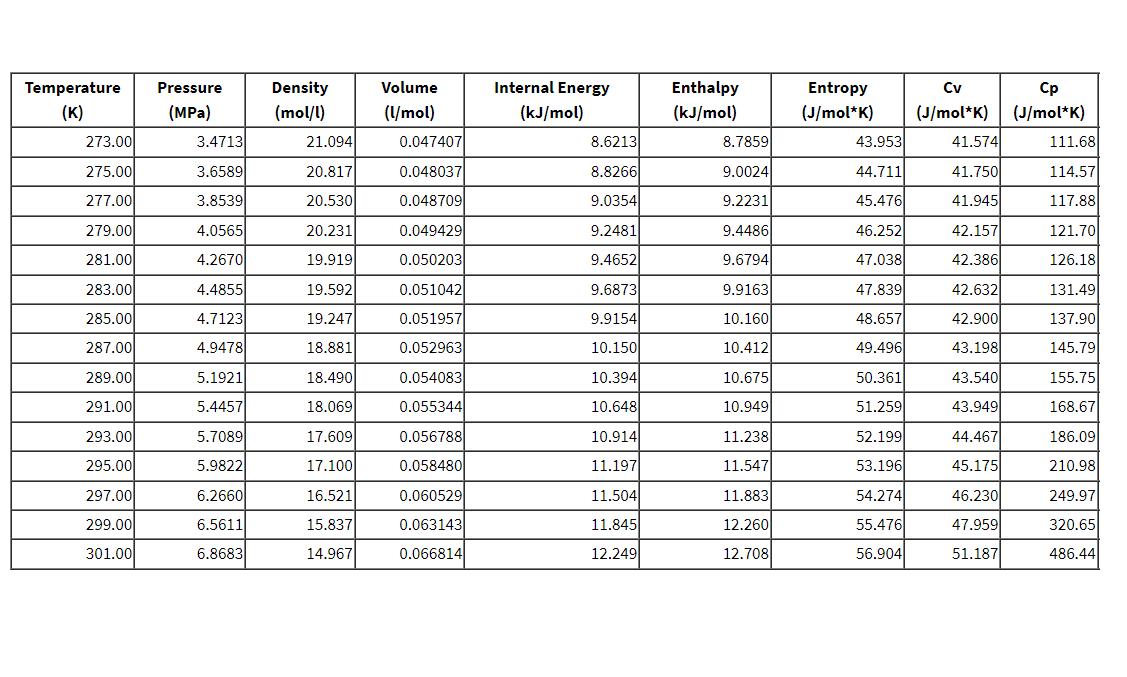
\includegraphics[scale=0.75]{Problem_2/Liquid_phase.png}
    
%     \label{fig:enter-label}
% \end{figure}

\begin{center}
\footnotesize{
\begin{tabular}{|>{\centering\arraybackslash}m{2cm}|>{\centering\arraybackslash}m{2cm}|>{\centering\arraybackslash}m{2cm}|>{\centering\arraybackslash}m{2cm}|>{\centering\arraybackslash}m{2cm}|>{\centering\arraybackslash}m{2cm}|}
    \hline
    Nhiệt độ & Áp suất & Mật độ mol & Nội năng & Enthalpy & Entropy \\
    $(\si{K})$ & $(\si{MPa})$ & $(\si{mol/l})$ & $(\si{kJ/mol})$ & $(\si{J/mol \cdot K})$ & $(\si{J/mol \cdot K})$ \\
    \hline
    273.00 & 3.4713 & 21.094 & 8.6213 & 8.7859 & 43.953 \\
    \hline
    275.00 & 3.6589 & 20.817 & 8.8266 & 9.0024 & 44.711 \\
    \hline
    277.00 & 3.8539 & 20.530 & 9.0354 & 9.2231 & 45.476 \\
    \hline
    279.00 & 4.0565 & 20.231 & 9.2481 & 9.4486 & 46.252 \\
    \hline
    281.00 & 4.2670 & 19.919 & 9.4652 & 9.6794 & 47.038 \\
    \hline
    283.00 & 4.4855 & 19.592 & 9.6873 & 9.9163 & 47.839 \\
    \hline
    285.00 & 4.7123 & 19.247 & 9.9154 & 10.160 & 48.657 \\
    \hline
    287.00 & 4.9478 & 18.881 & 10.150 & 10.412 & 49.496 \\
    \hline
    289.00 & 5.2921 & 18.490 & 10.394 & 10.675 & 50.361 \\
    \hline
    291.00 & 5.4457 & 18.069 & 10.648 & 10.949 & 51.259 \\
    \hline
    293.00 & 5.7089 & 17.609 & 10.914 & 11.238 & 52.199 \\
    \hline
    295.00 & 5.9822 & 17.100 & 11.197 & 11.547 & 53.196 \\
    \hline
    297.00 & 6.2660 & 16.521 & 11.504 & 11.883 & 54.274 \\
    \hline
    299.00 & 6.5611 & 15.837 & 11.845 & 12.260 & 55.476 \\
    \hline
    301.00 & 6.8683 & 14.967 & 12.249 & 12.708 & 56.904 \\
    \hline
\end{tabular}
}
\end{center}

\begin{flushright}
    (Biên soạn bởi Yuki)
\end{flushright}
\setcounter{equation}{0}
% \begin{center}
%     \normalcolor{\textbf{Bài giải}}
% \end{center}
% \begin{enumerate}[label=\textbf{\alph*,}]\itemsep0em
\item Theo nguyên lý 1 nhiệt động lực học:
\begin{equation} \label{eq1_P2_d1}
    T dS = dU + pdV.
\end{equation}
Ta nhớ rằng nội năng khí lý tưởng tuân theo biểu thức:
\begin{equation} \label{eq2_P2_d1}
    dU = C_V dT = \frac{R}{\gamma-1} dT.
\end{equation}
Phương trình Clapeyron-Mendeleev cho $\SI{1}{mol}$ khí lý tưởng: 
\begin{equation} \label{eq3_P2_d1}
    p=\frac{RT}{V}.
\end{equation}
Thay các phương trình (\ref{eq2_P2_d1}) và (\ref{eq3_P2_d1}) vào phương trình (\ref{eq1_P2_d1}) rồi chia hai vế cho $T$, ta được
\begin{equation} \label{eq4_P2_d1}
    dS = \frac{R}{\gamma-1} \frac{dT}{T} + R \frac{dV}{V}.
\end{equation}
Lấy nguyên hàm phương trình (\ref{eq4_P2_d1}), ta thu được hàm entropy của khối khí là một hàm trạng thái chỉ phụ thuộc vào $T$ và $V$:
\begin{equation} \label{eq5_P2_d1}
    S(T,V)= \frac{R}{\gamma-1} \ln (T) + R \ln (V) + S_0.
\end{equation}
Với $S_0$ là một hằng số.

\item Ta biết rằng, các quá trình đoạn nhiệt là các quá trình đẳng entropy (entropy không đổi), chúng sẽ là những đường thẳng đứng vuông góc với trục hoành trên đồ giản đồ $T$-$S$. Còn các quá trình đẳng nhiệt sẽ là các đường nằm ngang vuông góc với trục tung $T$, mỗi đường giãn đẳng nhiệt làm thể tích tăng $n_i$ lần được biểu diễn trên giản đồ $T$-$S$ này, theo biểu thức (\ref{eq5_P2_d1} sẽ ứng với một đoạn có độ dài $\Delta S_i = R \ln (n_i)$. Như vậy ta thu được đồ thị:

\begin{center}
\begin{tikzpicture}[>=stealth]
    %Vẽ hệ trục toạ độ 
    \draw[->](0,2.0)--(13,2.0);
    \draw[->](0,2.0)--(0,8.0);
    \draw (13,2) node[above]{$S$} (0,8.0) node[left]{$T$} (0,2.0) 
    node[below left]{$O$};
    %Vẽ đồ thị
    \draw[->] (3,7.0)--(4,7.0);
    \draw[->] (4,7.0)--(4,6.5);
    \draw[->] (4,6.5)--(5,6.5);
    \draw[->] (5,6.5)--(5,6.0);
    \draw[->] (5,6.0)--(6,6.0);
    \draw[->] (6,6.0)--(6,5.5);
    \draw[->] (6,5.5)--(7,5.5);
    \draw[->] (7,5.5)--(7,5.0);
    \draw[->] (7,5.0)--(8,5.0);
    \draw[->] (8,5.0)--(8,4.5);
    \draw[->] (8,4.5)--(9,4.5);
    \draw[->] (9,4.5)--(9,4.0);
    \draw[->] (9,4.0)--(10,4.0);
    \draw[->] (10,4.0)--(10,3.5);
    \draw[->] (10,3.5)--(3,3.5);
    \draw[->] (3,3.5)--(3,7.0);
    %Nhiệt độ 
    \draw (3.5,7.0) node[above]{$T_1$};
    \draw (4.5,6.5) node[above]{$T_2$};
    \draw (5.5,6.0) node[above]{$T_3$};
    \draw (6.5,5.5) node[above]{$T_4$};
    \draw (7.5,5.0) node[above]{$T_5$};
    \draw (8.5,4.5) node[above]{$T_6$};
    \draw (9.5,4.0) node[above]{$T_7$};
    \draw (6.5,3.5) node[above]{$T_8$};
    %Ghi chú \Delta S.
    \draw[dashed] (7,5.0)--(7,2.0);
    \draw[dashed] (8,5.0)--(8,2.0);
    \draw (7.5,2.0) node[below]{$\Delta S_i = R \ln (n_i)$};
\end{tikzpicture}
\end{center}


\item Ta có thể xác định được hiệu entropy giữa điểm đầu và điểm cuối của quá trình nén đẳng nhiệt thông qua 2 con đường của đồ thị. Gọi tỷ số thể tích giữa trạng thái đầu và trạng thái cuối của quá trình nén đẳng nhiệt là $n_8$. Ta có thể xác định được hiệu entropy giữa điểm đầu và điểm cuối của quá trình co đẳng nhiệt thông qua 2 con đường của đồ thị:
\begin{equation} \label{eq6_P2_d1}
    \begin{split}
        & R \ln (n_1) + R \ln (n_2) + ... + R \ln (n_6) + R \ln (n_7) = R \ln (n_8) \ \ \ (= \Delta S_8) \\
        & \Rightarrow n_8 = n_1 n_2 n_3 n_4 n_5 n_6 n_7 \approx 1.60.
    \end{split}
\end{equation}

\item Việc tính công của chu trình này thông qua việc tính tổng công của từng quá trình nhỏ tương đối phức tạp. Song, ta hoàn toàn có thể thay thế công việc này thông qua tính tổng nhiệt lượng khí nhận nhiệt $Q_1$ và tống nhiệt lượng khí nhả ra $Q_2$ rồi xác định công của khối khí thực hiện là $W'=Q_1-Q_2$.

Theo định nghĩa của entropy nhiệt động lực học, ta dễ dàng có thể lấy nó ở dạng tích phân trong trường hợp này:
\begin{equation} \label{eq7_P2_d1}
    Q = \sum T_i \Delta S_i.
\end{equation}
Áp dụng công thức trên, ta tìm được:
\begin{equation} \label{eq8_P2_d1}
    Q_1 = T_1 R \ln (n_1) + T_2 R \ln (n_2) + T_3 R \ln (n_3) +...+ T_6 R \ln (n_6) + T_7 R \ln (n_7).
\end{equation}
Và 
\begin{equation} \label{eq9_P2_d1}
    Q_2 = T_8 R \left[ \ln (n_1) + \ln (n_2) + \ln (n_3) +...+ \ln(n_6) + \ln (n_7)  \right].
\end{equation}
Vậy công khí thực hiện trong quá trình là:
\begin{equation} \label{eq10_P2_d1}
    W'= Q_1 - Q_2 = \sum_{i=1}^7 R \left( T_i - T_8 \right) \ln (n_i) = \SI{179}{J}.
\end{equation}
Hiệu suất của chu trình:
\begin{equation} \label{eq11_P2_d1}
    H = 1 - \frac{Q_2}{Q_1} = 1 - \frac{\displaystyle T_8 \sum_{i=1}^7 \ln (n_1)}{\displaystyle \sum_{i=1}^7 T_i \ln (n_i)} = 13.1 \%.
\end{equation}

\end{enumerate}

\textbf{Biểu điểm} 
\begin{center}
\begin{tabular}{|>{\centering\arraybackslash}m{1cm}|>{\raggedright\arraybackslash}m{14cm}| >{\centering\arraybackslash}m{1cm}|}
    \hline
\textbf{Phần} & \textbf{Nội dung} & \textbf{Điểm} \\
    \hline
    \textbf{a} & Tìm được hàm entropy $S(T,V)$ (\ref{eq5_P2_d1}) & $0.50$ \\
    \hline
    \textbf{b} & Vẽ phác đồ thị & $1.00$ \\
    \hline
    \textbf{c} & Tính được $n_8$ (\ref{eq6_P2_d1}) & $1.00$ \\
    \hline
    \textbf{d} & Tính $Q_1$ (\ref{eq8_P2_d1}) & $0.50$ \\
    \cline{2-3}
    & Tính công $W'$ (\ref{eq10_P2_d1}) & $0.50$ \\ 
    \cline{2-3}
    & Tính hiệu suất $H$ (\ref{eq11_P2_d1}) & $0.50$ \\
    \hline
\end{tabular}
\end{center}

\noindent \textbf{Mở rộng vấn đề:} \\
Đây là một bài toán lấy ý tưởng từ bài 2 ngày 1 VPhO 2022 (một bài toán cũng thường xuất hiện trong các sách bài tập vật lý đại cương). Không khó để nhận thấy, việc mở rộng bài toán từ 3 cặp đường đẳng nhiệt và đoạn nhiệt lên thành 8 cặp đường không phải là chỉ để tăng sự phức tạp trong tính toán mà còn đòi hỏi người giải phải tìm ra được quy luật tổng quát của bài toán với số cặp đường đẳng nhiệt và đoạn nhiệt là bất kì. Phần \textbf{a} và \textbf{b} của bài toán đã được đưa vào với mục đích dẫn dắt đến một lời giải đơn giản hơn so với cách làm thường thấy. \\
Lời giải này đưa đến 2 thủ thuật nho nhỏ:
\begin{enumerate}
    \item Đôi khi entropy cho phép ta đơn giản hoá các vấn đề trong tính toán (đặc biệt là trong các bài toán có các quá trình đẳng nhiệt và đoạn nhiệt).
    \item Đôi khi, việc tính công của quá trình trở nên phức tạp hơn việc xác tìm nhiệt lượng thu $Q_1$ và nhiệt lượng toả $Q_2$.
\end{enumerate}
Hiển nhiên, các thủ thuật kia chỉ có thể dùng từ "đôi khi", khá nhiều khi chúng phản tác dụng và việc sử dụng chúng hiệu quả không sẽ phụ thuộc vào kinh nghiệm của người giải. Cho một số ứng dụng đơn giản, hãy thử những mẹo trên và mở rộng bài toán này cho $p$ quá trình giãn và $q$ quá trình co, giải lại các bài toán về chu trình Carnot, chu trình Otto, chu trình Atkinson, chu trình Stirling,... chúng có thể không mang đến một lời giải hoàn hảo như ở bài toán này, song chúng vẫn có những hiệu quả nhất định khi sử dụng.

Đây chỉ là một bài toán mang tính giáo dục cũng như đưa ra các cách giải quyết vấn đề thú vị chưa được sử dụng nhiều trong các tài liệu Olympiad, các số liệu trong bài toán chỉ nhằm mục đích kiểm tra đáp số đơn giản hơn, không có ý nghĩa thực tế.


\newpage
{\normalcolor\textbf{CÂU 3.}}\vspace{1.5mm}

\setcounter{equation}{0}
% \textbf{Định lý Earnshaw và thấu kính tĩnh điện}

% Một vòng dây điện tích \(Q\) hình đa giác đều \(n\) cạnh có bán kính đường tròn ngoại tiếp \(R\). Trục \(\Delta\) là trục đi qua tâm và vuông góc với mặt phẳng vòng dây có dạng đối xứng trụ.

% \ \ 

% \textbf{1.} Chứng minh rằng, điện trường ở gần trục \(\Delta\).

% \ \ 

% \textbf{2.} Tính vector điện trường \(\mathbf{E}\) tại một vị trí gần trục \(\Delta\).

% \ \ 

% Theo định lý Earnshaw, một hệ điện tích trong chân không không thể tạo ra một điểm cân bằng bền chỉ bởi các tương tác tĩnh điện.

% \ \  

% \textbf{3.} Chỉ ra rằng trong bài toán này, vị trí cân bằng không thể là vị trí cân bằng bền với mọi chuyển động.

% \ \ 

% \textbf{4.} Bắn một hạt điện tích \(q\) khối lượng \(m\) với vận tốc \(v_0\) song song với trục \(\Delta\) và cách trục \(\Delta\) một khoảng \(b\) (với \(b \ll R\) ). Quỹ đạo của hạt điện tích đi qua vòng dây điện tích giống như một tia sáng đi qua thấu kính có tiêu cự \(f\). Tính tiêu cự \(f\) này theo \(n\), \(R\), \(Q\), \(q\), \(\varepsilon_0\), \(m\) và \(v_0\).

\textbf{Hiệu ứng bề mặt} \footnote{Skin effect.}

Hiệu ứng bề mặt là một hiệu ứng xuất hiện phổ biến trong các các đường mạch điện truyền dẫn dòng điện cao tần. Theo đó, thay vì phân bố đều trên toàn dây dẫn như các dòng điện tần số thấp, ở tần số cao, các dòng điện tập trung chủ yếu ở sát bề mặt kim loại và nhanh chóng giảm theo độ sâu với cấp số mũ.

\ \

\textbf{1. Mô hình mạch tương đương đơn giản}

Quy luật chuyển động của dòng điện trong một vật dẫn với hằng số điện môi \(\mu\) và điện trở suất \(\rho\) có thể được mô tả bởi một mạch điện tương đương (như hình \ref{fig:Equivalent_circuit_skin_effect}) \footnote{Điện kháng \(L_0\) được sử dụng để mô tả hằng số từ thẩm trong chân không \(\mu_0\) của môi trường ngoài. Ta không cần quan tâm đến nó trong bài toán này}. Ở hình \ref{fig:Equivalent_circuit_skin_effect}A, phân bố dòng điện trong tấm vật liệu được tương đương như một mạch điện vô hạn, theo đó, từng khối chữ nhật có chiều dài \(l\), chiều rộng \(w\) và độ dày \(\Delta z\) (như hình \ref{fig:Conductor}) được tương đương như một mắt mạch tương đương gồm một thành phần cảm kháng \(\Delta L\) và một phần điện dẫn \footnote{Nghịch đảo của điện trở.} \( \Delta G \).

\begin{figure}[!h]
    \centering
    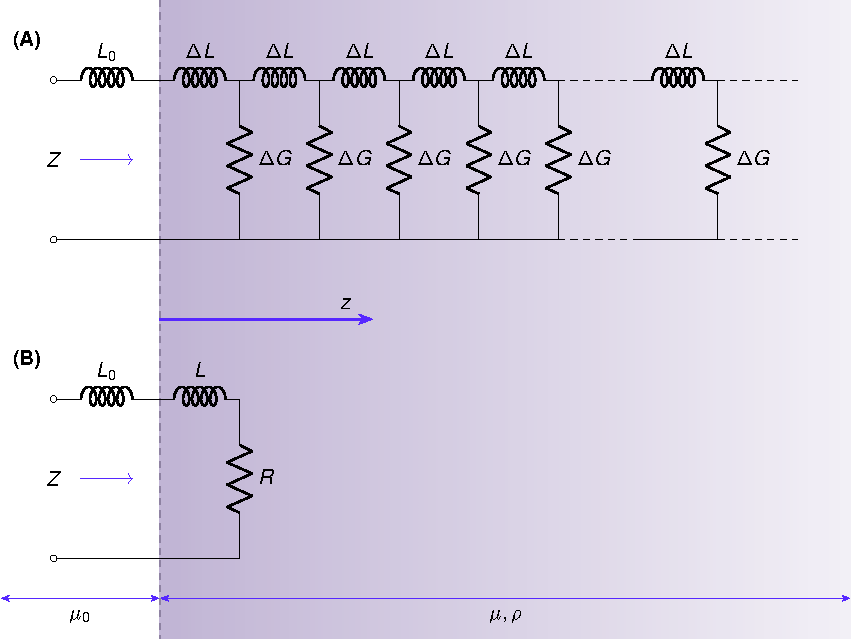
\includegraphics[width=0.9\textwidth]{Problem_3/Figs_P3/Equivalent_circuit_skin_effect.pdf}
    \caption{Mô hình mạch tương đương của hiệu ứng bề mặt. (A) Mạch tương đương phân bố vô hạn trong không gian. (B) Mạch tương đương trở kháng của mạch.}
    \label{fig:Equivalent_circuit_skin_effect}
\end{figure}

Dựa vào các tính toán mạch tương đương, mạng mạch vô hạn tuần hoàn trên có trở kháng quan sát từ phía bề mặt ngăn cách hai môi trường là \(Z\) và có thể được phân tích như tổng của hai phân tử \(R\) và \(L\) (như hình \ref{fig:Equivalent_circuit_skin_effect}B).

\begin{figure}
    \centering
    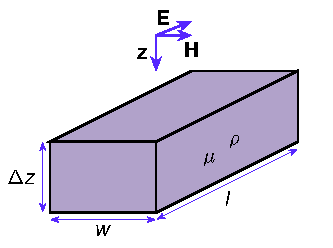
\includegraphics[width=0.6\textwidth]{Problem_3/Figs_P3/Conductor.pdf}
    \caption{Mô hình một phần tử trong khối vật dẫn.}
    \label{fig:Conductor}
\end{figure}

\textbf{Câu hỏi a.} Tìm \( \Delta L \) và \( \Delta G \) của mạch trong mô hình mạch tương đương vô hạn theo \(\mu\), \(\rho\), \(w\), \(l\) và \( \Delta z \).

\ \

\textbf{Câu hỏi b.} Tìm các thông số trở kháng \(Z\), \(R\) và \(L\) theo \(\mu\), \(\rho\), \(w\), \(l\) và tần số \(\omega\) của dòng điện.

\ \

\textbf{Câu hỏi c.} Độ sâu bề mặt\footnote{Skin depth.} là độ sâu để biên độ dòng điện giảm đi \(e\) lần. Xác định độ sâu bề mặt của tấm vật liệu theo tần số \(\omega\) của dòng điện, độ từ thẩm \(\mu\) và điện trở suất \(\rho\).

\ \

\textbf{2. Điện trở gây bởi hiệu ứng bề mặt}

\ \

\textbf{Câu hỏi d.} Chứng minh rằng, ta có thể tính điện trở \(R\) tương đương của một đoạn vật dẫn điện chịu ảnh hưởng bởi hiệu ứng bề mặt có thể tính theo công thức:
\begin{equation}
    R = \dfrac{1}{\mu_0} \dfrac{\partial L_0}{\partial z} R_S,
\end{equation}
trong đó
\begin{itemize}
    \item \(L_0\) là độ tự cảm của một miếng bề mặt vật dẫn được xét với giả thiết độ sâu bề mặt bằng không.
    \item Tọa độ \(z\) được hiểu là tọa độ có trục vuông góc với bề mặt.
    \item \(R_S = \sqrt{\omega \mu \rho/2}\) được gọi là hệ số điện trở suất bề mặt.
\end{itemize}

\ \

\textbf{Câu hỏi e.} Tính điện trở gây ra bởi hiệu ứng bề mặt đối với hai ống dây dẫn tròn có chiều dài \(l\), bán kính \(a\) và có trục dây đặt cách nhau một khoảng \(2b\).
\setcounter{equation}{0}
% \begin{center}
%     \normalcolor{\textbf{Bài giải}}
% \end{center}
% \begin{enumerate}[label=\textbf{\alph*,}]\itemsep0em
\item Theo tính đối xứng cầu của hệ, ta có thể dễ dàng suy ra mật độ dòng
\begin{equation} \label{eq1_P3_d1}
    j(r) = \frac{I}{2\pi h r}.
\end{equation}
Một hạt electron chuyển động đến vị trí có bán kính $r$ sẽ nhận được một công $eV(r)$ của điện trường, xem rằng công này được chuyển hoá làm tăng động năng của hạt điện tích $\frac{1}{2}mv^2$, từ đó ta xác định được vận tốc của hạt:
\begin{equation} \label{eq2_P3_d1}
    \frac{1}{2}mv^2 = eV(r) \Rightarrow v(r)= \sqrt{ \frac{2eV(r)}{m} }.
\end{equation}
Theo định nghĩa mật độ dòng:
\begin{equation} \label{eq3_P3_d1}
    j(r) = \rho v \Rightarrow \rho = \frac{j}{v} = \frac{I}{2\pi h r} \sqrt{ \frac{m}{2eV} } .
\end{equation}

\item Trong hệ đối xứng cầu, cường độ điện trường tại bán kính $r$ là
\begin{equation} \label{eq4_P3_d1}
    E = - \frac{dV}{dr}.
\end{equation}
Áp dụng định luật Gauss cho một vỏ trụ bán kính $r$ và độ dày $dr$, ta có
\begin{equation} \label{eq5_P3_d1}
    \begin{split}
        E(r+dr) \cdot 2 \pi h (r+dr) - E(r) \cdot 2 h \pi r &= \frac{\rho}{\varepsilon_0} \cdot 2 \pi h r dr \\
        \Rightarrow \frac{d}{dr} \left( E \cdot r \right) = \frac{\rho}{\varepsilon_0} r.
    \end{split}
\end{equation}
Từ (\ref{eq4_P2_d1}) và (\ref{eq5_P3_d1}), ta được:
\begin{equation} \label{eq6_P3_d1}
    \frac{1}{r} \frac{d}{dr} \left( r \frac{dV}{dr} \right) = \frac{\rho}{\varepsilon_0}.
\end{equation}
\item Từ (\ref{eq3_P2_d1}) và (\ref{eq6_P3_d1}) ta thu được phương trình vi phân của $V(r)$:
\begin{equation} \label{eq7_P3_d1}
    \frac{d}{dr} \left( r \frac{dV}{dr} \right) = \frac{I}{2\pi \varepsilon_0 h} \sqrt{ \frac{m}{2eV} } .
\end{equation}
Thế dạng nghiệm $V(r)=Ar^\alpha$ vào phương trình (\ref{eq7_P3_d1}), ta được:
\begin{equation} \label{eq8_P3_d1}
    A \alpha^2 r^{\alpha-1} = \frac{I}{2 \pi \varepsilon_0 h} \sqrt{ \frac{m}{2e A} } r^{-\alpha/2}.
\end{equation}
Đồng nhất hệ số 2 vế, ta được:
\begin{equation} \label{eq9_P3_d1}
    \alpha-1=-\frac{\alpha}{2} \Rightarrow \alpha = \frac{2}{3}.
\end{equation}
Và 
\begin{equation} \label{eq10_P3_d1}
    A \alpha^2 = \frac{I}{2 \pi \varepsilon_0 h} \sqrt{ \frac{m}{2e A} } \Rightarrow A= \left( \frac{9I}{8\pi \varepsilon_0 h} \sqrt{\frac{m}{2e}} \right)^{2/3}.
\end{equation}
\item Thay (\ref{eq9_P3_d1}) và (\ref{eq10_P3_d1}) vào công thức nghiệm
\begin{equation} \label{eq11_P3_d1}
    V(r) = \left( \frac{9I}{8\pi \varepsilon_0 h} \sqrt{\frac{m}{2e}} \right)^{2/3} r^{2/3}.
\end{equation}
Tại $r=R$ thì $V(R)=U$ nên
\begin{equation} \label{eq12_P3_d1}
    U = \left( \frac{9I}{8\pi \varepsilon_0 h} \sqrt{\frac{m}{2e}} \right)^{2/3} R^{2/3}.
\end{equation}
Hay
\begin{equation} \label{eq13_P3_d1}
    I = \left( \frac{8\pi \varepsilon_0 h}{9R} \sqrt{ \frac{2e}{m} }\right) U^{3/2}.
\end{equation}
Như vậy
\begin{equation} \label{eq14_P3_d1}
    K = \frac{8\pi \varepsilon_0 h}{9R} \sqrt{ \frac{2e}{m} } .
\end{equation}
\end{enumerate}

\textbf{Biểu điểm} 
\begin{center}
\begin{tabular}{|>{\centering\arraybackslash}m{1cm}|>{\raggedright\arraybackslash}m{14cm}| >{\centering\arraybackslash}m{1cm}|}
    \hline
\textbf{Phần} & \textbf{Nội dung} & \textbf{Điểm} \\
    \hline
    \textbf{a} & Tìm được mật độ dòng $j$ theo $I$ (\ref{eq1_P3_d1}) & $0.25$ \\
    \cline{2-3}
    & Tìm vận tốc $v$ theo điện thế $V$ (\ref{eq2_P3_d1}) & $0.50$ \\
    \cline{2-3}
    & Tìm mật độ điện khối $\rho$ theo $V$ và $r$ (\ref{eq3_P3_d1}) & 0.25 \\
    \hline
    \textbf{b} & Viết biểu thức điện trường theo điện thế (\ref{eq4_P3_d1}) & $0.25$ \\
    \cline{2-3}
    & Áp dụng định luật Gauss cho vỏ trụ (\ref{eq5_P3_d1}) & $0.50$ \\
    \cline{2-3}
    & Kết hợp 2 phương trình để viết được phương trình vi phân (\ref{eq6_P3_d1}) & 0.25 \\
    \hline
    \textbf{c} & Hoàn chỉnh phương trình vi phân (\ref{eq7_P3_d1}) & $0.25$ \\
    \cline{2-3}
    & Thế dạng nghiệm của phương trình (\ref{eq8_P3_d1}) & $0.25$ \\
    \cline{2-3}
    & Tính được $\alpha$ (\ref{eq9_P3_d1}) & $0.50$ \\
    \cline{2-3}
    & Tính được $A$ (\ref{eq10_P3_d1}) & $0.50$ \\ 
    \hline
    \textbf{d} & Thay điều kiện biên và viết được $U$ theo $I$ (\ref{eq12_P3_d1}) & $0.25$ \\ 
    \cline{2-3}
    & Tính hệ số $K$ (\ref{eq14_P3_d1}) & $0.25$ \\
    \hline
\end{tabular}
\end{center}

\noindent \textbf{Mở rộng vấn đề:} \\
Đây là một bài toán không có các tính toán phức tạp nhưng khá khó để nhìn được ra đường hướng giải quyết, đòi hỏi người giải cần có một kiến thức nền khá tốt. Đối với những người đã học tương đối sâu về phân bố của điện từ trường và biết sử dụng các công cụ toán tốt, không khó để nhận thấy câu hỏi phần \textbf{b} chính là chứng minh phương trình Poisson $\Delta V = \frac{\rho}{\varepsilon_0}$ đối với hệ toạ độ trụ có tính đối xứng trụ, đây là một phương trình được dẫn ra từ 2 trong 4 phương trình Maxwell, 1 phương trình là định luật Gauss về thông lượng của điện trường và 1 phương trình về lưu số của điện trường (liên hệ giữa điện trường và điện thế). Tổng quát hơn, với mọi bài toán về tĩnh điện và các hệ từ trường dừng, ta sẽ đều cần sử dụng 1 phương trình về thông lượng và 1 phương trình về lưu số để giải quyết chúng. \\
Bài toán diot chân không và định luật Child-Langumuir được lấy từ Bài tập giải sẵn "Diode chân không" trang 59-60 quyển \textit{Điện từ học 2} của Jean Marie Brébec (bộ sách PFIEV), bản dịch của Lê Băng Xương, Nhà xuất bản giáo dục Việt Nam. Bài toán được tham khảo thêm từ bài 2.53 trang 109 trong quyển sách \textit{Introduction to Electrodynamics} của David Griffiths cũng như các bài báo về "Child-Langumuir law". \\
Như ta có thể thấy, bài toán diode chân không này phổ biến nhất là trường hợp 2 bản tụ phẳng rộng có diện tích $S$ đặt song song cách nhau một khoảng $d$ như trong bài 2.53 quyển \textit{Introduction to Electrodynamics}. Kết quả của bài toán này sẽ là:
$$ I = \frac{4 \varepsilon_0 S}{9d^2} \sqrt{ \frac{2e}{m}} U^{3/2}.$$
Các vấn để mở rộng cho bài toán này như khảo sát trường hợp electron có vận tốc ban đầu $v_0$ đáng kể cũng được được xét tới trong các bài báo \href{https://arxiv.org/abs/physics/0411175v1}{Generalization of Child-Langmuir Law for Non-Zero Injection Velocities in a Planar} và \href{http://de.arxiv.org/abs/1506.07417v1}{A new approach to the Child-Langmuir law}. 

Bài toán của chúng ta là dạng hình trụ của diode, tất nhiên, ta hoàn toàn có thể mở rộng bài toán này cho trường hợp hệ diode hình cầu, song nó đưa đến một phương trình vi phân tương đối phức tạp và không phù hợp để giải ở đây.

\newpage
{\normalcolor \textbf{CÂU 4.}}\vspace{1.5mm}

\setcounter{equation}{0}
\textbf{Khuếch đại thuật toán}

Bộ khuếch đại thuật toán (OPerational AMPlifier), hay còn gọi là OPAMP là một linh kiện điện tử dùng để thực hiện một số phép toán như cộng, trừ, nhân, chia, tích phân, đạo hàm,... khi nó kết hợp với các linh kiện bên ngoài.

Một OPAMP cơ bản có cấu tạo gồm 8 chân, nhưng trong khuôn khổ bài này, chúng ta chỉ xét một OPAMP như hình vẽ


\begin{figure}[h]
\centering
\begin{subfigure}[t]{0.3\textwidth}
\centering
\begin{circuitikz} 
    \draw
     (0,0) node[op amp] (opamp) {}
     (opamp.+) node[left] {$v_+$}
     (opamp.-) node[left] {$v_-$}
     (opamp.out) node[right] {$v_o$}
     (opamp.up) --++(0,0.5) node[vcc]{$V_+$}
     (opamp.down) --++(0,-0.5) node[vee]{$V_-$};
    \end{circuitikz}
 \caption{Ký hiệu OPAMP}
 \end{subfigure}
 %
\begin{subfigure}[t]{0.6\textwidth}
 \centering
 \begin{circuitikz}[american,scale=0.73,font=\footnotesize]
 \ctikzset{bipoles/length=11mm} 
    \draw
        (0,4) to[short, -o] ++(-1.7,0) node[shift={(-0.4,0)}] {$v_-$}
        (-1.7, 3.6) to [short, -*] (-1.7, 3.6) node[ground]{}
        (0,0) to[short, -o] ++(-1.7,0) node[shift={(-0.4,0)}] {$v_+$}
        (-1.7,-0.4) to [short, -*] (-1.7,-0.4) node[ground]{}
        (0,4) to[resistor, l=$R_\text{in}$] (0,0)
        (1.5,0.5) to [short,-*] (1.5,0.5) node[ground]{} to [cV, invert, l_=$A(v_+ - v_-)$] ++(0,1.5) to [resistor, l=$R_\text{out}$] ++(5.5,0) to [short, -o] ++(0.1,0) node[shift={(0.4,0)}] {$v_\text{o}$}
        (-1,-2) to [short] ++(0,8) to [short] (6.5,2) to [short] (-1,-2) 
        (-1.7, 3) node[below,shift={(-0.,0)} ] {$v_G=0$}
    ;\end{circuitikz}
 \caption{Mạch tương đương của OPAMP}\label{opampcircuit}
 \end{subfigure}
 \caption{OPAMP}
 \end{figure}


Trong đó hai chân $V_+$ và $V_-$ dùng để cấp nguồn cho thiết bị, khi có hai điện thế $v_+$ và $v_-$ được đặt lần lượt vào hai đầu vào không đảo ngược và đảo ngược thì ở đầu ra sẽ xuất hiện một điện thế $v_0$ sao cho:
\begin{equation}
    v_0=A(v_+-v_-) \ \ ,
\end{equation}
trong đó A được gọi là "độ lợi vòng lặp hở" đặc trưng với từng loại OPAMP. Thiết bị này có thể được miêu tả bằng mô hình mạch điện \subref{opampcircuit}, trong đó ký hiệu của nguồn $A(v_+ - v_-)$ gọi là nguồn áp phụ thuộc, tức là độ lớn của nó phụ thuộc vào một đại lượng khác(ở đây là hiệu điện thế giữa hai đầu vào của OPAMP). 




Trong thực tế, OPAMP thường được kết hợp với một số linh kiện ngoài như điện trở, tụ điện hoặc cuộn cảm để phản hồi giữa đầu ra và đầu vào, giúp cho chúng ta có thể điều chỉnh được độ lợi của OPAMP bằng cách điều chỉnh các thông số thiết bị ngoài.
\begin{enumerate}
    \item Tìm độ lợi vòng lặp đóng $\dfrac{v_\text{o}}{v_\text{s}}$ cho mạch dưới đây. Áp dụng với LM741 có độ lợi vòng lặp mở $2 \times 10^5$, điện trở đầu vào $2 \si{M\Omega}$ và điện trở đầu ra $50 \si{\Omega}$ và $R_f=200 \si{\Omega}$, $R_1=100 \si{\Omega}$.
\end{enumerate}
\begin{center}
    \begin{circuitikz}[american]\draw
(0,0) node[op amp] (opamp) {}
 (opamp.+)  to [short] ++ (-1.5,0) to [short] ++(0,-2) node[ground]{} 
 (opamp.-) to [R,l_={$R_1$},i_<=$i_1$] ++(-3,0) to [V, l_=$v_\text{s}$] ++(0,-3) to [short,-o] ++(6,0) node[right]{$-$}
 (opamp.out) to [short,-o] ++(0.62,0) node[right] {$+$}
 (1.64,-1.3) node[right]{$v_o$}
 (opamp.-) to [short]++(-0.5,0) to [short] ++(0,1) to [R,l={$R_f$},i>=$i_f$] ++(2.9,0) to (opamp.out)
 (opamp.-) node[above left]{I}
 (opamp.out) node[above right]{O}
;\end{circuitikz}
\end{center}

Tiếp theo đây, để cho đơn giản, ta coi các OPAMP là lý tưởng, nghĩa là điện trở đầu vào rất lớn, điện trở đầu ra rất nhỏ và độ lợi vòng lặp hở rất lớn. Khi đó $v_1 \approx v_2$ và dòng điện ở hai đầu vào OPAMP $i_-=i_+=0$.
\begin{enumerate}[resume]
    \item Tìm tỉ số $\dfrac{v_o}{v_s}$ với mạch trên khi OPAMP là lý tưởng.    
\end{enumerate}
Xét ba mạch OPAMP có dạng như hình vẽ:
\begin{figure}[h]
\begin{subfigure}[t]{0.6\textwidth}
\centering
\begin{circuitikz}[american,scale=1]
\draw
(-2,0) node[op amp] (opamp) {}
 (opamp.+) to [short] ++ (-1.5,0) to [short] ++(0,-2) node[ground]{} 
 (opamp.-) to [short] ++(-4.5,0) to[R,l_={$R_2$}] ++(0,-1.5)to [V, l_=$v_\text{2}$] ++(0,-1.5)
 (opamp.-) to [short] ++(-3,0) to[R,l_={$R_1$}] ++(0,-1.5)to [V, l_=$v_\text{1}$] ++(0,-1.5)
 (opamp.-) to [short] ++(-6,0) to[R,l_={$R_3$}] ++(0,-1.5)to [V, l_=$v_\text{3}$] ++(0,-1.5) to [short,-o] ++(9,0) node[right]{$-$}
 (opamp.out) to [short,-o] ++(0.62,0) node[right] {$+$}
 (-0.5,-1.3) node[]{$v_\text{sum}$}
 (opamp.-) to [short] ++(0,1) to [R,l={$R_f$},i>=$i_f$] ++(2.4,0) to (opamp.out)
;\end{circuitikz}
 \caption{Mạch cộng}
 \end{subfigure}
 %
\begin{subfigure}[t]{0.4\textwidth}
 \centering
 \begin{circuitikz}[american,font=\small]\draw
(0,0) node[op amp] (opamp) {}
 (opamp.+) to [short] ++ (-1.5,0) to [V,l=$v_s$] ++(0,-2) node[ground]{} 
 (opamp.-) to [R,l_={$R$}] ++(-3,0) to [short] ++(0,-3) to [short,-o] ++(6,0) node[right]{$-$}
 (opamp.out) to [short,-o] ++(0.62,0) node[right] {$+$}
 (1.64,-1.3) node[right]{$v_\text{ni}$}
 (opamp.-) to [short] ++(0,1) to [R,l={$R_f$},i>=$i_f$] ++(2.4,0) to (opamp.out)
 ;\end{circuitikz}
 \caption{Mạch khuếch đại không đảo}
 \end{subfigure}\\[1ex]
\begin{subfigure}{\linewidth}  
\centering
 \begin{circuitikz}[american]\draw
(0,0) node[op amp] (opamp) {}
 (opamp.+) to [short] ++ (-1.5,0) to [short] ++(0,-2) node[ground]{} 
 (opamp.-) to [R,l_={$R$}] ++(-3,0) to [V, l=$v_\text{s}$] ++(0,-3) to [short,-o] ++(6,0) node[right]{$-$}
 (opamp.out) to [short,-o] ++(0.62,0) node[right] {$+$}
 (1.64,-1.3) node[right]{$v_\text{int}$}
 (opamp.-) to [short] ++(0,1) to [C,l={$C$},i>=$i_f$] ++(2.4,0) to (opamp.out)
  ;\end{circuitikz}
 \caption{Mạch tích phân}
 \end{subfigure}
 \end{figure}

\begin{enumerate}[resume]
    \item Tìm $v_\text{sum}$ ,$v_\text{int}$ và $v_\text{ni}$ ứng với ba mạch.
    \item Từ các mạch trên, thiết lập mạch điện để giải phương trình vi phân sau:
    \begin{equation}
        a\dfrac{d^2x}{dt^2}+b\dfrac{dx}{dt}+cx=d ,
    \end{equation}
với điều kiện ban đầu $\dot{x}(0)=e$, $x(0)=f$ .
    \item Đề xuất một cách thiết kế để tạo ra một phần tử mạch điện có giá trị "điện trở âm" ($V_{in}/I_{in} < 0$) bằng các điện trở, OPAMP và nối đất.  
\end{enumerate}

\begin{flushright}
    (Biên soạn bởi Hiagari)
\end{flushright}


\setcounter{equation}{0}
% \begin{center}
%     \normalcolor{\textbf{Bài giải}}
% \end{center}
% \textbf{1.} \textbf{a,} Sơ đồ tạo ảnh:
\begin{align}
     S_1 \xrightarrow[\displaystyle \infty \quad F]{\displaystyle F} S_2 \xrightarrow[\displaystyle L -F \quad l- f]{\displaystyle f_0} S_3 \xrightarrow[\displaystyle  f \quad \infty]{\displaystyle f} S_4.
\end{align}


Ta có phương trình tạo ảnh của thấu kính trường là
\begin{align}
\frac{1}{f_0} &= \frac{1}{L - F} + \frac{1}{d_0 - f}\\
\Leftrightarrow L &= F + \frac{f_0 (l - f)}{l - f - f_0} = 1177.5 \mathrm{~mm}.\label{41}
\end{align}

\textbf{b,} Độ bội giác của hệ ba thấu kính là
\begin{align}
    G_\infty = \frac{F}{f} \frac{l - f}{L - F} = \frac{F}{f} \left( 1 + \frac{f-l}{f_0} \right)  = \frac{160}{3} \approx 53.33.
\end{align}

\textbf{2.} Ta có sơ đồ tạo ảnh của \textit{vật kính} qua hệ thị kính:
\begin{align}
     S_1 \xrightarrow[\displaystyle L \quad d']{\displaystyle f_0} S_2 \xrightarrow[\displaystyle l - d' \quad \Delta]{\displaystyle  f} S_3.
\end{align}

Ta có hệ phương trình thấu kính:
\begin{align}
    \frac{1}{f_0} &= \frac{1}{L} + \frac{1}{d'}.\\
    \frac{1}{f} &= \frac{1}{l - d'} + \frac{1}{\Delta}.
\end{align}

Kết hợp với phương trình (\ref{41}) và giải hệ ba phương trình ta thu được kết quả
\begin{align}
    \Delta = f \left[\frac{1}{1 + \dfrac{f}{f_0 - l}} + \frac{f}{F} \frac{1}{\left(1 + \dfrac{f-l}{f_0} \right)^2} \right] =\frac{507}{64} \approx 7.92 \mathrm{~mm}.
\end{align}

Đường kính vòng tròn ánh sáng xuất hiện trên đồng tử mắt người là
\begin{align}
    \delta = -\frac{D}{G_\infty} = -\frac{39}{16} = -2.4375 \mathrm{mm}.
\end{align}

Ta thấy rằng $\delta$ bé hơn kích thước đồng tử mắt người, nên người có thể nhìn được toàn bộ ánh sáng qua hệ.

\vspace{1mm}

\textbf{3.} Để xác định thị trường qua kính thiên văn, ta coi mắt người là nguồn sáng điểm rồi tìm ảnh của mắt qua hệ thấu kính. Ta có sơ đồ tạo ảnh
\begin{align}
     S_1 \xrightarrow[\displaystyle \Delta \quad d_1]{\displaystyle f} S_2 \xrightarrow[\displaystyle l - d_1 \quad d_2]{\displaystyle f_0} S_3 \xrightarrow[\displaystyle  L - d_2 \quad d_3]{\displaystyle F} S_4.
\end{align}
Ta có hệ phương trình thấu kính
\begin{align}
    \frac{1}{f} &= \frac{1}{\Delta} + \frac{1}{d_1}.\\
    \frac{1}{f_0} &= \frac{1}{l - d_1} + \frac{1}{d_2}.\\
    \frac{1}{F} &= \frac{1}{L - d_2} + \frac{1}{d_3}.
\end{align}
Bấm máy thay số liệu ta thu được
\begin{align}
    d_1 &= -7.5\mathrm{~mm}\\
    d_2 &= -225 \mathrm{~mm}\\
    d_3 &=8311.11 \mathrm{~mm}
\end{align}

Giả sử từ mắt nhìn qua được toàn bộ thấu kính mắt. Khi đó đường kính vòng tròn nhìn được trên kính trường là $d_0'$, khi đó
\begin{align}
    \Big| \frac{d_1}{l -d_1} \Big| &= \frac{d}{d_0'}\\
    \Rightarrow d_0' &= 75 \mathrm{~mm} > d_0 = 30 \mathrm{~mm}
\end{align}

Nhận thấy rằng mắt người không thể nhận toàn bộ ánh sáng qua kính mắt.

Làm tương tự đối với kính trường, ta tìm được vòng tròn ánh sáng trên vật kính, gọi là $D'$, khi đó
\begin{align}
    \Big|\frac{d_2}{L - d_2} \Big| &= \frac{d_0}{D'}\\
    \Rightarrow D' &= 187 \mathrm{~mm} > D =130 \mathrm{mm}
\end{align}

Từ đó ta nhận định rằng ánh sáng đi qua toàn bộ vật kính sẽ không bị mất mát năng lượng khi đi đến mắt người, và \textit{không ngược lại}.

\vspace{1mm}
Từ đó ta tìm được góc mở thị trường khi nhìn qua kính thiên văn là 
\begin{align}
    \theta \approx \frac{D}{d_3} = 0.01564\mathrm{~rad}.
\end{align}
Đường kính góc của Mặt Trăng khi nhìn từ Trái Đất là 
\begin{align}
    \theta_M = \frac{2R_M}{d_{ME}} = 0.00900 \mathrm{~rad}.
\end{align}
Cuối cùng, ta xác định được tỉ lệ diện tích của Mặt Trăng so với trường nhìn qua kính thiên văn là
\begin{align}
    k = \left( \frac{\theta_M}{\theta} \right)^2 = 33.4 \%.
\end{align}



 \textbf{Biểu điểm} 
\begin{center}
\begin{tabular}{|>{\centering\arraybackslash}m{1cm}|>{\raggedright\arraybackslash}m{14cm}| >{\centering\arraybackslash}m{1cm}|}
    \hline
    \textbf{Phần} & \textbf{Nội dung} & \textbf{Điểm} \\
    \hline
    \textbf{a} & Viết được biểu thức chữ và giá trị số của $L$ & 0.50\\   
    \cline{2-3}
    &  Viết được biểu thức chữ và giá trị số của $G_\infty$& 0.50\\
    \hline
    \textbf{b} & Tìm được biểu thức chữ và giá trị của $\Delta$ & 1.00 \\
        \cline{2-3}
        & Tìm được $\delta$ & 0.50 \\
    \hline
    \textbf{c} & Tìm được $d_1,d_2,d_3$ & 0.50\\
    \cline{2-3}
    & Chứng minh được toàn bộ ánh sáng qua vật kính khi đến mắt không bị mất mát & 0.50\\
    \cline{2-3}
    & Tìm được tỉ số $k$ & 0.50\\
    \hline
\end{tabular}
\end{center}

\newpage
{\normalcolor \textbf{CÂU 5.}}\vspace{1.5mm}

\setcounter{equation}{0}
\textbf{Nguyên lý Cực đại Entropy và Đàn chim Bay}

Vật lý hiện diện trong thế giới quanh ta, giúp mô tả các hành vi quần thể của những hệ thống tương tác phức tạp, từ đám khí lý tưởng đến đám đông người. Trong bài tập này, chúng ta sẽ cùng khám phá xem nguyên lý cực đại entropy đã được áp dụng như thế nào để thành lập lên một trong những lý thuyết Vật Lý Sinh thành công nhất hiện đại dùng để mô tả đàn chim bay (xem hình \ref{fig:Bird}A).

\begin{figure}[!h]
    \centering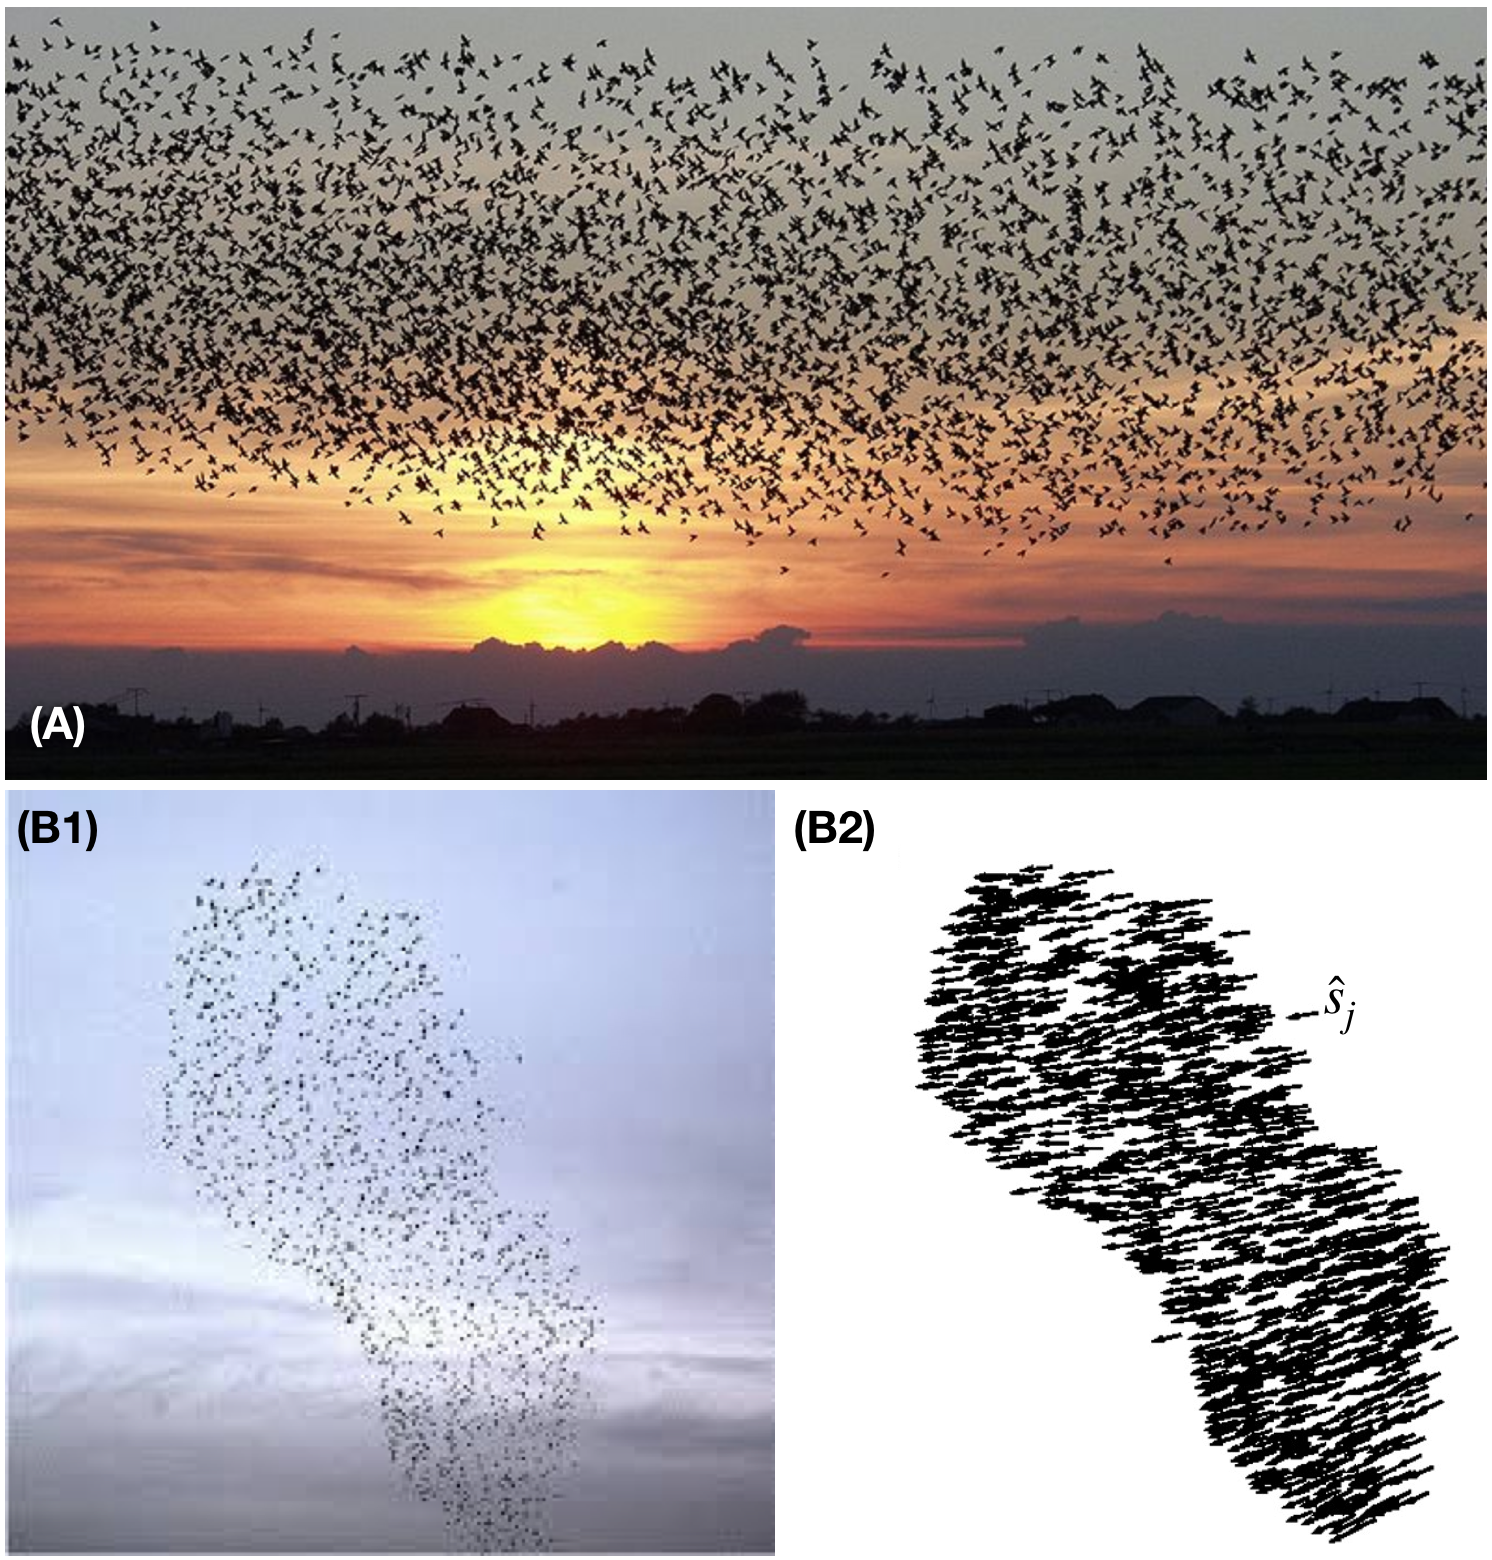
\includegraphics[width=0.96\textwidth]{Problem_5/Figs_P5/fig01.png}
    \caption{(A) Đàn chim bay. (B) Mô tả Toán học của một đàn chim bay, với (B1) là hình ảnh thô của đàn chim và (B2) là tập hợp các vector hướng bay của các cá thể trong đàn chim tại cùng thời điểm.}
    \label{fig:Bird}
\end{figure}

Nguyên lý cực đại entropy là một phương pháp thống kê dùng để suy ra phân phối xác suất không thiên vị nhất có thể dựa trên thông tin đã biết, đồng thời tránh đưa ra giả định về những điều chưa biết. Về cơ bản, nguyên lý này nói rằng, với một tập hợp các ràng buộc đã biết (như giá trị trung bình), phân phối xác suất tốt nhất là phân phối có entropy cao nhất mà vẫn thỏa mãn các ràng buộc này. Ở đây, công thức entropy thường được sử dụng là Boltzmann-Gibbs-Shannon entropy.

\ \ 

Với xác suất xảy ra của một đại lượng Vật Lý liên tục $X$, Boltzmann-Gibbs-Shannon entropy $S$ được xác định bởi giá trị trung bình của hàm \textit{độ ngạc nhiên} $I(x)=-\ln\left[ p(x)\right]$ theo biến $x$:
\begin{equation}
    S = \langle I \rangle = - \int_{\Omega_X} dx \ p(x) \ln\left[ p(x)\right] \ ,
\end{equation}
trong đó $x$ đại diện cho kết quả đo của đại lượng $X$, $p(x)$ là xác suất đo đại lượng $X$ cho ra kết quả $x$,  $\Omega_X$ là vùng khả dĩ của các kết quả đo cho đại lượng $X$.

\ \  

Chúng ta sẽ cùng nhau tìm hiểu về những ứng dụng của nguyên lý này trong việc diễn giải các kết quả thí nghiệm Vật lý, khi trong báo cáo chỉ cung cấp ít các thông tin liên quan.

\ \  

\textbf{1. Phương pháp nhân Lagrange}

Trước hết, chúng ta cùng nhau tìm hiểu về một phương pháp Toán học, vô cùng mạnh mẽ và hiệu quả, giúp chúng ta giải quyết các vấn đề tìm kiếm quỹ tích các điểm cực trị trong bối cảnh có ràng buộc -- phương pháp nhân Lagrange.

\ \ 

Xét việc tìm cực trị của hàm số $f(\vec{z})$ theo biến $\vec{z}\equiv [z_1, z_2, ..., z_{n_z}]$ (trong đó $n_z$ là số lượng các biến), với các điều kiện ràng buộc $C_k(\vec{z})$=0 (trong đó $k=1,2,...,n_C$, và $n_C$ là số lượng điều kiện ràng buộc). Hàm Lagrangian có thể được thiết lập như sau:
\begin{equation}
    L(\vec{Z}) = f(\vec{z}) - \sum_{k=1}^{n_C} \lambda_k C_k(\vec{z}) \ ,
\end{equation}
với biến $\vec{Z} \equiv [\vec{z}, \lambda_1, \lambda_2, \lambda_3, ..., \lambda_{n_C}]$.

\ \ 

\textbf{Câu hỏi a.} Hãy chứng minh rằng, điều kiện cực trị của hàm số $L(\vec{Z})$ theo biến $\vec{Z}$ có thể giúp chúng ta xác định được quỹ tích các điểm cực trị $\vec{z}$ của hàm số $f(\vec{z})$ dưới các ràng buộc $C_k(\vec{z})$.

\ \  

Những câu hỏi tiếp theo đây đều có thể được giải quyết sử dụng phương pháp nhân Lagrange.

\ \  

\textbf{2. Các hàm phân bố nội suy}

Để tránh rườm rà, nhiều báo cáo kết quả thí nghiệm thường không cung cấp toàn bộ dữ liệu thô từ các phép đo, mà chỉ trình bày giá trị ước lượng tốt nhất cùng với độ phân tán của các kết quả, thể hiện qua giá trị trung bình và phương sai.

\ \  

Hãy xác định hàm phân bố nội suy $p(x)$ cho xác suất thu được kết quả $x$ khi đo đại lượng $X$ thỏa mãn nguyên lý cực đại entropy, khi chúng ta chỉ biết những tính chất sau đây:

\ \  

\textbf{Câu hỏi b.} Vùng khả dĩ $\Omega_X$ là miền số thực i.e. $x\in (-\infty,\infty)$, giá trị đo trung bình của $X$ là $\mu$ và giá trị phương sai của $X$ là $\sigma^2 > 0$. Biểu diễn $p(x)$ theo $\mu$, $\sigma^2$, và biến $x$.

\ \  

\textbf{Câu hỏi c.} Vùng khả dĩ $\Omega_X$ là miền số dương i.e. $x\in[0,\infty)$, và giá trị đo trung bình của $X$ là $\mu$ (với $\mu > 0$). Biểu diễn $p(x)$ theo $\mu$ và biến $x$.

\ \  

Bây giờ, chúng ta sẽ áp dụng những kiến thức này vào một hệ vật lý cụ thể. Xét một quần thể gồm nhiều bậc tự do khác nhau mang năng lượng, e.g. một đám khí lý tưởng được cấu tạo từ nhiều phân tử khí khác nhau. Chúng ta sẽ tìm hiểu về tính chất thống kê của kết quả $\mathcal{E}$ khi đo giá trị năng lượng $E$ trên mỗi bậc tự do này.

\ \  

\textbf{Câu hỏi d.} Vùng khả dĩ $\Omega_E$ là miền chặn dưới i.e. $x\in[\mathcal{E}_{\min},\infty)$, và giá trị đo trung bình của $E$ là $\mathcal{E}_0$ (với $\mathcal{E}_0 > \mathcal{E}_{\min}$). Hãy chứng minh rằng, xác suất $p(\mathcal{E})$ -- cho kết quả $\mathcal{E}$ khi đo đại lượng $E$ -- thỏa mãn nguyên lý cực đại entropy chính là hàm phân bố Maxwell-Boltzmann:
\begin{equation}
    p(\mathcal{E}) \propto \exp\left( -\beta \mathcal{E} \right) \ \ ,
\end{equation}
trong đó $\beta$ là một hằng số nào đó liên hệ trực tiếp với $\mathcal{E}_0$.

\ \  

\textbf{3. Vật Lý Sinh mô tả đàn chim bay}

Có lẽ các bạn đã biết, hàm phân bố Maxwell-Boltzmann tạo ra cầu nối giữa hành vi ở cấp độ cá nhân và hành vi ở cấp độ quần thể, đặc biệt hiệu quả khi áp dụng cho những hệ Vật Lý được cấu tạo từ các cá thể đơn giản và vô tri. Tuy nhiên, với các hệ Vật Lý thường thấy trong thế giới Sinh học, nơi các cá thể có khả năng quan sát, xử lý thông tin và ra quyết định, để xây dựng cầu nối này thì hàm phân bố cần được sử dụng sẽ phải rất khác biệt.

\ \  

Xét một đàn chim bay, với chú chim $j$ ở vị trí $\vec{r}_j(t)$ và đang bay với vận tốc $\vec{v}_j(t)=d\vec{r}_j(t)/dt$ ($t$ là thời điểm hiện tại). Hướng bay của chú chim này được xác định bởi
$\hat{s}_j(t) = \vec{v}_j(t)/\left| \vec{v}_j(t)\right|$ (xem các hình \ref{fig:Bird}B), trong đó $\left|\vec{\circ}\right|$ là giá trị độ dài của vector $\vec{\circ}$. Định nghĩa giá trị liên kết $C_{jk}$ giữa cặp chim $j$ và $k$ theo giá trị trung bình của tích vô hướng hướng bay $\hat{s}_j(t) \cdot \hat{s}_k(t)$ theo thời gian $t$. Khi $C_{jk}$ càng gần với $1$, thì có nghĩa rằng cặp chim này càng cố gắng bay cùng hướng với nhau hơn.

\ \ 

Giả sử đàn chim bao gồm $N\gg 1$ chú chim, thế thì $j=1,2,3,...,N$ và mỗi \textit{vi thái} $\Theta$ của hướng bay đàn chim này có thể được xác đinh bởi $N$ các giác trị véc-tơ:
$$ \Theta \equiv \left[ \hat{s}_1, \hat{s}_2, \hat{s}_3, ..., \hat{s}_N \right] \ .$$
Cho biết tập hợp giá trị tất cả các hàm liên kết hướng bay $\{ C_{ij} \}$, chúng ta muốn xác định xác suất $p(\Theta)$ ở thời điểm bất kỳ quan sát được đàn chim bay đang sở hữu \textit{vi thái} $\Theta$.

\ \ 

\textbf{Câu hỏi e.} Chứng minh rằng:
\begin{equation}
    p(\Theta) \propto \exp\left[ -\frac12 \sum^N_{j=1} \sum^N_{k=1} \beta_{jk} \left(\hat{s}_j \cdot \hat{s}_k \right) \right] \ ,
\end{equation}
với mỗi giá trị $\beta_{jk}$ có thể được xác định từ tập hợp tất cả các giá trị liên kết hướng bay $\{ C_{jk}\}$.

\ \ 

Chú ý rằng, để đơn giản hóa câu hỏi ở trên, chúng ta xét ràng buộc là tất cả các tất cả các giá trị liên kết $C_{jk}$. Các nhà Vật Lý Sinh sử dụng ít ràng buộc hơn (chỉ với các cặp chim \textit{đủ gần} nhau) nhưng chặt hơn (tất cả các giá trị liên kết này đều bằng nhau). Nói cách khác, khi khớp lý thuyết này với thực nghiệm, thì chỉ có đúng hai giá trị tự do là kích thước hàng xóm $n$ và giá trị liên kết trong nhóm hàng xóm $C$. Kích thước hàng xóm $n$ xác định nhóm hàng xóm \textit{đủ gần} với một chú chim. Cụ thể, chim $j$ được coi là \textit{đủ gần} chim $k$ nếu nó nằm trong số $n$ chim gần nhất quanh chim $k$. Ý nghĩa sinh học ở đây là mỗi con chim đưa ra quyết định dựa trên quan sát và tương tác với các chim trong nhóm hàng xóm của mình, tập trung vào các tương tác địa phương thay vì toàn bộ bầy. Mô hình đơn giản này mô tả rất tốt những hành vi quần thể của nhiều bầy đàn sinh vật di cư đồng bộ khác nhau, e.g. bầy chim sáo đá châu Âu (\textit{Sturnus vulgaris}, xem hình \ref{fig:Sturn}) với $n\approx 11$ và $C\approx 0.996$. 

\begin{figure}[!h]
    \centering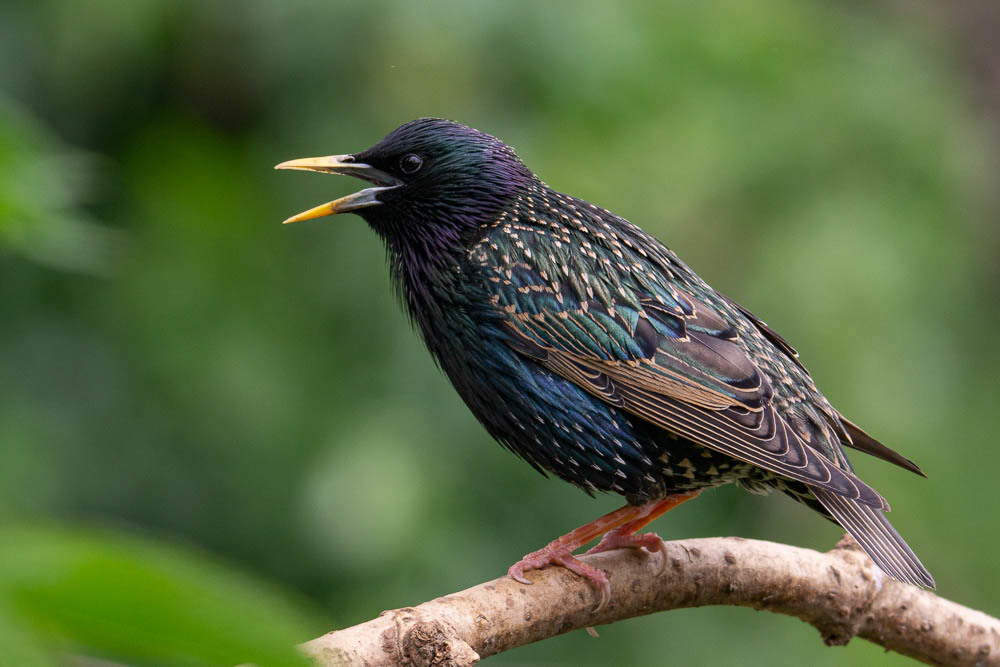
\includegraphics[width=0.6\textwidth]{Problem_5/Figs_P5/fig02.jpg}\caption{Một chú chim sáo đá châu Âu (\textit{Sturnus vulgaris}).}
    \label{fig:Sturn}
\end{figure}

\ \ 

\setcounter{equation}{0}
% \begin{center}
%     \normalcolor{\textbf{Bài giải}}
% \end{center}
% \begin{enumerate} 
    \item  \textbf{Enzyme cứng hay mềm ?}\\
    \begin{enumerate}[label=\textbf{\alph*,}]\itemsep0em
        \item Giả sử abzyme biến dạng một lượng $x_1$ và cơ chất biến dạng một lượng $x_2$. Từ trạng thái chuyển tiếp như hình vẽ trong đề bài, cơ chất liên kết với vùng hoạt động, do đó:
        \begin{equation} \label{eq1_enzyme}
            a+x_1=2d-x_2.
        \end{equation}
        Mặt khác, ta có định luật 3 Newton cho cân bằng lực ở vùng hoạt động:
        \begin{equation} \label{eq2_enzyme}
            k_e x_1 = k_s x_2.
        \end{equation}
        Từ phương trình (\ref{eq1_enzyme}) và phương trình (\ref{eq2_enzyme}), ta suy ra $x_1$ và $x_2$:
        \begin{equation} \label{eq3_enzyme}
        \begin{split}
            x_1=\dfrac{k_s}{k_e+k_s}(2d-a),\\
            x_2=\dfrac{k_e}{k_e+k_s}(2d-a).
        \end{split}
        \end{equation}
        Năng lượng cung cấp cho enzyme gây ra biến dạng của enzyme là:
        \begin{equation} \label{eq4_enzyme}
            E_e=\dfrac{1}{2}k_e x_1^2 =  \dfrac{k_e k_s^2}{2(k_e+k_s)^2}(2d-a)^2. 
        \end{equation}
        Năng lượng cung cấp cho cơ chất gây ra biến dạng của cơ chất là:
        \begin{equation} \label{eq5_enzyme}
            E_s=\dfrac{1}{2}k_s x_2^2 =  \dfrac{k_s k_e^2}{2(k_e+k_s)^2}(2d-a)^2. 
        \end{equation}
    \item Lấy phương trình (\ref{eq4_enzyme}) chia cho phương trình (\ref{eq5_enzyme}), ta thu được liên hệ về năng lượng:
    \begin{equation} \label{eq6_enzyme}
        \dfrac{E_e}{E_s}=\dfrac{k_s}{k_e}.
    \end{equation}
    Như ta đã biết, một enzyme xúc tác càng hiệu quả sẽ tiêu tốn càng ít năng lượng cho việc biến dạng chính nó, hay chính là $E_e \ll E_s$, tương đương với $k_e \gg k_s$. Do đó, một enzyme hoạt động hiệu quả sẽ phải thật "cứng" để phần lớn năng lượng được sử dụng vào biến dạng của cơ chất, từ đó thúc đẩy phản ứng hoá học.\\
    \textit{Trong mô hình này, ta xét abzyme do abzyme chỉ dùng tương tác van der Waals, các enzyme tự nhiên sử dụng cả liên kết cộng hoá trị nên "cứng" hơn nhiều abzyme, do đó mà khả năng xúc tác phản ứng cũng mạnh hơn nhiều lần.}
    \end{enumerate}
    \item \textbf{Bỏ qua động năng?}\\
    \begin{enumerate}[label=\textbf{\alph*,}]\itemsep0em
        \item Phương trình động lực học:
        \begin{equation} \label{eq7_enzyme}
        \begin{split}
            m\dfrac{d^2 x}{dt^2}&=F_{\text{ela}}\\
            \rho V \dfrac{d^2 x}{dt^2}&= - \dfrac{ES}{D}x \\
            \dfrac{d^2 x}{dt^2}+&\dfrac{E}{\rho D^2}x=0.    
        \end{split}
        \end{equation}
        Đặt $\dfrac{E}{\rho D^2}=\omega_0^2$, phương trình (\ref{eq7_enzyme}) trở thành:
        \begin{equation} \label{eq8_enzyme}
            \dfrac{d^2 x}{dt^2}+\omega_0^2 x=0.
        \end{equation}
        Chu kỳ dao động của enzyme:
        \begin{equation} \label{eq9_enzyme}
            T_0=\dfrac{2\pi}{\omega_0}=2\pi \sqrt{\dfrac{\rho D^2}{E}}=2.51 \times 10^{-11} \ \si{s}.
        \end{equation}
        \item 
        \begin{enumerate}
            \item Ta có phương trình động lực học như sau:
        \begin{equation} \label{eq10_enzyme}
        \begin{split}
            m\dfrac{d^2 x}{dt^2} &=F_{\text{vis}}+F_{\text{ela}}\\
            \rho V \dfrac{d^2 x}{dt^2} &=-10 \eta D \dfrac{dx}{dt} - \dfrac{ES}{D}x \\
            \dfrac{d^2 x}{dt^2}+ &\dfrac{10\eta }{\rho D^2}\dfrac{dx}{dt}+\dfrac{E}{\rho D^2}x=0.
        \end{split}
        \end{equation}
        Đặt $\dfrac{10\eta }{\rho D^2}=2\beta$, phương trình (\ref{eq10_enzyme}) trở thành:
        \begin{equation} \label{eq11_enzyme}
            \dfrac{d^2 x}{dt^2}+2\beta\dfrac{dx}{dt}+\omega_0^2 x=0.
        \end{equation}
        Trong đó:
        \begin{equation} \label{eq12_enzyme}
            \beta = \dfrac{5\eta}{\rho D^2}=3.125\times 10^{11} \ \si{s^{-1}}, \quad \omega_0=\sqrt{\dfrac{E}{\rho D^2}}=2.5\times 10^{11}\ \si{s^{-1}}.
        \end{equation}
        Phương trình vi phân (\ref{eq10_enzyme}) có nghiệm là:
        \begin{equation} \label{eq13_enzyme}
            x(t)=Ae^{\lambda_1t}+Be^{\lambda_2t}.
        \end{equation}
        Trong đó:
        \begin{align} \label{eq14_enzyme}
            \lambda_1&=-\beta+\sqrt{\beta^2-\omega_0^2}=-1.25\times 10^{11} \ \si{s^{-1}},\\
            \label{eq15_enzyme}
            \lambda_2&=-\beta-\sqrt{\beta^2-\omega_0^2}=-5\times 10^{11} \ \si{s^{-1}}.
        \end{align}
        Tại $t=0$, $x(0)=x_0$ và $v(0)=x'(0)=0$, suy ra $A=\dfrac{\lambda_2 x_0}{\lambda_2-\lambda_1}=\dfrac{4}{3} x_0$ và $B=\dfrac{\lambda_1 x_0}{\lambda_1-\lambda_2}=-\dfrac{1}{3} x_0$.\\
        Nghiệm của phương trình vi phân (\ref{eq10_enzyme}) có thể viết lại thành:
        \begin{equation} \label{eq16_enzyme}
            x(t)=x_0\left(\dfrac{4}{3}e^{\lambda_1t}-\dfrac{1}{3}e^{\lambda_2t}\right).
        \end{equation}
        Trong đó $\lambda_1=-1.25\times 10^{11} \ \si{s^{-1}}$ và $\lambda_2=-5\times 10^{11} \ \si{s^{-1}}$.
    \begin{figure}[htp]
    \centering
    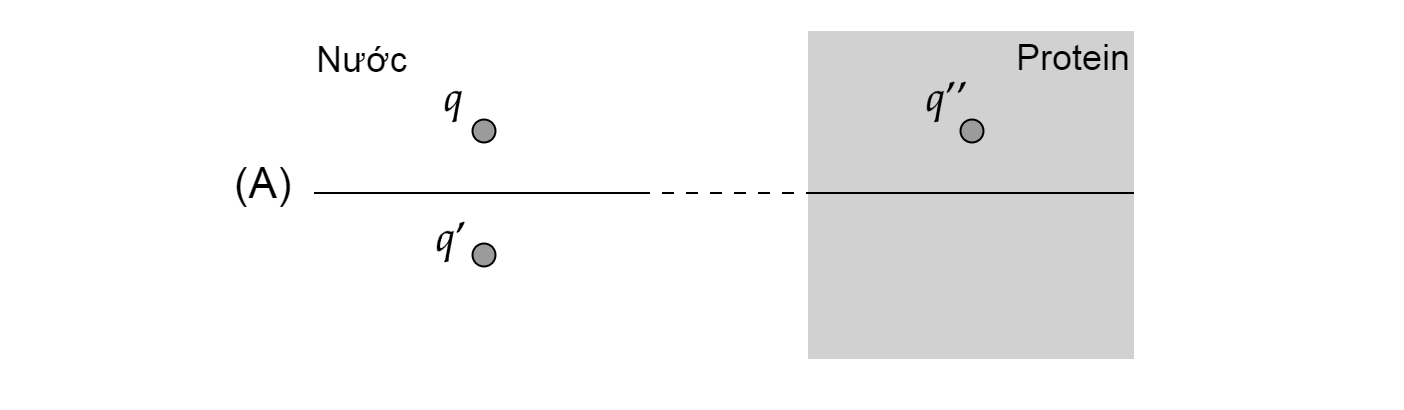
\includegraphics[scale=.27
        ]{Problem_5/image/3.png}
    \caption{Đồ thị $x(t)$.}
    \end{figure}
        \item Tại $t=T_0$, tỉ lệ giữa li độ $x$ và li độ $x_0$ ở thời điểm ban đầu:
        \begin{equation} \label{eq17_enzyme}
            N_1=\dfrac{x(T_0)}{x_0}=\dfrac{4}{3}e^{\lambda_1T_0}-\dfrac{1}{3}e^{\lambda_2T_0} \approx 5.78 \times 10^{-2}.
        \end{equation}
        Tại $t=2T_0$, tỉ lệ giữa li độ $x$ và li độ $x_0$ ở thời điểm ban đầu:
        \begin{equation} \label{eq18_enzyme}
            N_2=\dfrac{x(2T_0)}{x_0}=\dfrac{4}{3}e^{2\lambda_1T_0}-\dfrac{1}{3}e^{2\lambda_2T_0} \approx 2.51 \times 10^{-3}.
        \end{equation}
        
        \textit{Nhận xét: Ta thấy rằng động năng của enzyme bị phân tán và chuyển hoá thành nhiệt quá nhanh (thực tế là trước khi nó có thể được sử dụng trong quá trình xúc tác của enzyme). Quá trình dao động của enzyme hầu như không xảy ra hoặc bị tắt rất nhanh khi chúng ở trong nước (chưa kể đến môi trường nhớt hơn như màng). Do đó trong quá trình xúc tác của enzyme, ta bỏ qua động năng và coi enzyme tĩnh hoặc gần tĩnh.
        \newpage
        Qua bài tập này ta kết luận được hai tính chất rất đặc biệt của enzyme:
        \begin{enumerate}
            \item Năng lượng được cung cấp không phải để thay đổi cấu trúc enzyme mà phần lớn để đưa cơ chất vào enzyme và đưa nó vào trạng thái chuyển tiếp. Do đó vùng hoạt động của enzyme phải là cấu trúc cứng.
            \item Động năng không dùng trong quá trình xúc tác vì nó tiêu tán ra môi trường quá nhanh. Do đó có thể coi các mô hình là tĩnh hoặc gần tĩnh.
        \end{enumerate}}
        \end{enumerate}
    \end{enumerate}
\end{enumerate}

\textbf{Biểu điểm}
\begin{center}
\begin{tabular}{|>{\centering\arraybackslash}m{1cm}|>{\raggedright\arraybackslash}m{14cm}| >{\centering\arraybackslash}m{1cm}|}
    \hline
    \textbf{Phần} & \textbf{Nội dung} & \textbf{Điểm} \\
    \hline
    \textbf{1a} & Viết biểu thức cho $x_1$ và $x_2$ theo $k_e$, $k_s$, $d$ và $a$ (\ref{eq3_enzyme}) & $0.50$ \\
    \cline{2-3}
    &  Viết biểu thức cho $E_e$ theo $k_e$, $k_s$, $d$ và $a$ (\ref{eq4_enzyme}) & $0.25$ \\
    \cline{2-3}
    &  Viết biểu thức cho $E_s$ theo $k_e$, $k_s$, $d$ và $a$ (\ref{eq5_enzyme}) & $0.25$ \\
    \hline
    \textbf{1b} & Lập luận và kết luận & $0.25$ \\
    \hline
    \textbf{2a} & Dẫn ra phương trình vi phân (\ref{eq8_enzyme}) & $0.25$ \\
    \cline{2-3}
    & Tính được chu kỳ dao động $T$ (\ref{eq9_enzyme}) & $0.25$ \\
    \hline
    \textbf{2b.i} & Dẫn ra phương trình vi phân (\ref{eq10_enzyme}) & $0.25$ \\
    \cline{2-3}
    & Viết biểu thức $x(t)$ và các hệ số (\ref{eq16_enzyme}) & $1.25$ \\
    \hline
    \textbf{2b.ii} & Tính được tỉ lệ giữa li độ $x$ và $x_0$ tại thời điểm $t=T_0$ (\ref{eq17_enzyme}) & $0.25$ \\
    \cline{2-3}
    & Tính được tỉ lệ giữa li độ $x$ và $x_0$ tại thời điểm $t=2T_0$ (\ref{eq18_enzyme}) & $0.25$ \\
    \cline{2-3}
    & Lập luận và kết luận & $0.25$ \\
    \hline
\end{tabular}
\end{center}

%% Reference %%
\bibliographystyle{plain}
\begin{thebibliography}{}
\bibitem{bandaria2008} Jigar N. Bandaria, Samrat Dutta, Sarah E. Hill, Amnon Kohen, Christopher M. Cheatum (2008), \textit{Fast Enzyme Dynamics at the Active Site of Formate Dehydrogenase}, Journal of the American Chemical Society, 130(1), 22–23.           
\bibitem{giaotrinh} Nguyễn Thế Toàn, Nguyễn Hoạ Mi (2021), \textit{Giáo trình Vật lý Sinh học của Protein}, NXB ĐHQGHN.
\end{thebibliography}

\begin{center}
    \normalcolor{------------------------------------------------ HẾT ------------------------------------------------}
\end{center}

\end{document}